\documentclass[11pt]{article}

% =========================================================
% RTAS manuscript - compile-ready working LaTeX.
% Target journal: Scientometrics.
% Content and statistics frozen from the submission-clean manuscript.
% References: references_FINAL.bib
%
% This is a content-first working build. Before actual submission,
% migrate the content into the current Springer Nature sn-jnl template.
% =========================================================

\usepackage[margin=1in]{geometry}
\usepackage[T1]{fontenc}
\usepackage[utf8]{inputenc}
\usepackage{lmodern}
\usepackage{amsmath,amssymb}
\usepackage{booktabs}
\usepackage{threeparttable}
\usepackage{graphicx}
\usepackage{array}
\usepackage{microtype}
\usepackage{enumitem}
\usepackage{caption}
\usepackage{float}
\usepackage{hyperref}
\usepackage[
  backend=biber,
  style=authoryear,
  natbib=true,
  useprefix=true,
  sorting=nyt,
  sortcites=true,
  maxcitenames=2,
  maxbibnames=99,
  doi=true,
  url=false,
  isbn=false
]{biblatex}
\addbibresource{references_FINAL.bib}
\AtBeginBibliography{\small}

\hypersetup{
  colorlinks=true,
  linkcolor=black,
  citecolor=black,
  urlcolor=blue
}

\captionsetup{
  font=small,
  labelfont=bf,
  justification=justified,
  singlelinecheck=false
}

\graphicspath{{figures/}}

\title{\textbf{Measuring Research--Training Semantic Alignment:}\\
Project-Level Cross-Lingual Embeddings, Topic Prevalence Asymmetries, and Resource Concentration in Undergraduate Innovation Programs}

\author{
Author Name$^{1}$\\
\small $^{1}$Affiliation to be completed\\
\small Corresponding author: email@domain.edu
}
\date{}

\begin{document}
\maketitle

\begin{abstract}
Universities increasingly expect undergraduate research-training programs to reflect active faculty research, yet project-level alignment is rarely measured directly. We propose the Research--Training Alignment Score (RTAS), the mean cosine similarity between a student project-title embedding and unique OpenAlex-indexed articles assigned to the same college through advisor--author linkage. We apply RTAS to 3,714 undergraduate innovation projects (2020--2024) and 56,901 articles at Wuhan University; 33,312 articles (58.5\%) enter college-specific reference portfolios. Pairwise validation on 150 human-rated title pairs provides evidence of pairwise semantic validity (Spearman $\rho=0.405$; area under the ROC curve $=0.880$), supported by independent human raters, test--retest reliability, an LLM second rater, and lexical baselines. Mean RTAS differs by funding level (university 0.1212, provincial 0.1391, national 0.1460; $\eta^2=1.89\%$), but adjusted funding-level coefficients are not statistically distinguishable from zero. Joint BERTopic modeling (60,615 documents; 886 non-outlier topics) identifies 173 high-research/low-project and 10 low-research/high-project topics. Temporal onset is definable for 29/886 topics (3.27\%); among 24 definable high-research/low-project topics, median lag is $+0.5$ years. National-project allocation is concentrated (Gini $=0.746$; top 5\% share $=31.0\%$) and persistent (odds ratio $=2.06$, 95\% confidence interval [1.53, 2.76]), while project-level exposure to top-5\% advisors shows only a small mean RTAS difference that is not statistically distinguishable from zero ($d=0.083$, $p=0.065$). In the mixed model (intraclass correlation coefficient $=0.738$), advisor pre-project publication activity in the institution-linked OpenAlex corpus is positively associated with RTAS, whereas prior supervisory load is negatively associated. RTAS indexes semantic alignment, not training quality; estimates are observational.
\end{abstract}

\noindent\textbf{Keywords:} research--training alignment; undergraduate innovation; multilingual sentence embeddings; BERTopic; multilevel modeling; cumulative advantage

\section{Introduction}

\subsection{Motivation}

Research universities worldwide have made the integration of research and teaching a central policy goal, although the empirical relationship between research performance and teaching is neither automatic nor uniformly positive \citep{hattie1996relationship,healey2005linking,brew2003teaching,linn2015undergraduate}. At Wuhan University, undergraduate innovation projects are recorded at university, provincial, and national levels and are carried out under faculty supervision. This setting raises a scientometric question: whether the topics students pursue align with the research their colleges are actively publishing, and how funding level, advisor characteristics, and the concentration of supervisory resources relate to that alignment.

Existing work on research--teaching relationships operates mostly at the level of individual scholars or institutions, using performance composites and indicator correlations \citep{maisano2023empirical,scafetta2025rt,xiong2026nexus}. The scholar-level RT-score of \citet{scafetta2025rt}, for example, combines research and teaching performance into a faculty-level index. Scientometrics has long represented relations among documents through co-citation, bibliographic coupling, co-word analysis, topical networks, and publication-level classification \citep{small1973cocitation,boyack2010cocitation,callon1991coword,yanding2012networks,waltman2012classification}. More recent work extends this tradition with publication embeddings and semantic analysis \citep{lamers2021appraisal,huang2022interdisciplinarity,motohashi2024measuring}. What remains underdeveloped is a project-level measure of \emph{semantic} alignment: whether the content of a student project falls within the college's actual research portfolio. Such a measure must bridge languages (Chinese project titles; English article titles) and scale to tens of thousands of titles.

\subsection{This study}

We introduce RTAS (Research--Training Alignment Score), defined for each project as the mean cosine similarity between the multilingual sentence embedding of its title and the embeddings of the unique articles assigned to its college through advisor--author linkage over a cumulative window. RTAS is deliberately \emph{not} a performance ranking: it measures where student topics fall relative to the observed college research portfolio, not novelty, leadership, or impact.

We ask four research questions about the 2020--2024 cohorts of Wuhan University (40 colleges):
\begin{enumerate}[label=\textbf{RQ\arabic*.}]
\item \textbf{Heterogeneity.} Does RTAS differ by project funding level, and does the difference persist after accounting for college and advisor characteristics?
\item \textbf{Topic asymmetries and diffusion lags.} How are research-side and project-side topic prevalence distributed across quadrants, and where annual onset is identifiable on both sides, what lags are observed?
\item \textbf{Multilevel associations.} How much RTAS variance lies between colleges, and which advisor and project characteristics are associated with alignment?
\item \textbf{Concentration.} Is national project allocation concentrated and path-dependent across advisors, and does concentration coincide with higher alignment?
\end{enumerate}

A single-institution design is a deliberate choice: it holds the institutional setting and observation window constant while spanning 40 disciplinary organizations, creating a within-institution comparative setting for observing between-college variation at the cost of external validity (Sect.~\ref{sec:limitations}).

\subsection{Contributions}

The study makes three contributions. First, it provides a reproducible, project-level, cross-lingual semantic alignment measure with an explicit validity program (human raters, test--retest, a large language model [LLM] second rater, and lexical baselines) and a frozen aggregation choice. Second, it provides a static-prevalence quadrant decomposition of 886 research--training topics with threshold and clustering sensitivity checks, together with a conservative rule-based diffusion-lag analysis restricted to topics whose annual onset is definable on both sides. Third, it documents that raw funding-level differences are strongly attenuated after accounting for college and advisor context, while supervisory-resource concentration does not coincide with a statistically distinguishable mean alignment difference. Figure~\ref{fig:roadmap} summarizes the data tiers and analytical workflow.

\begin{figure}[H]
\centering
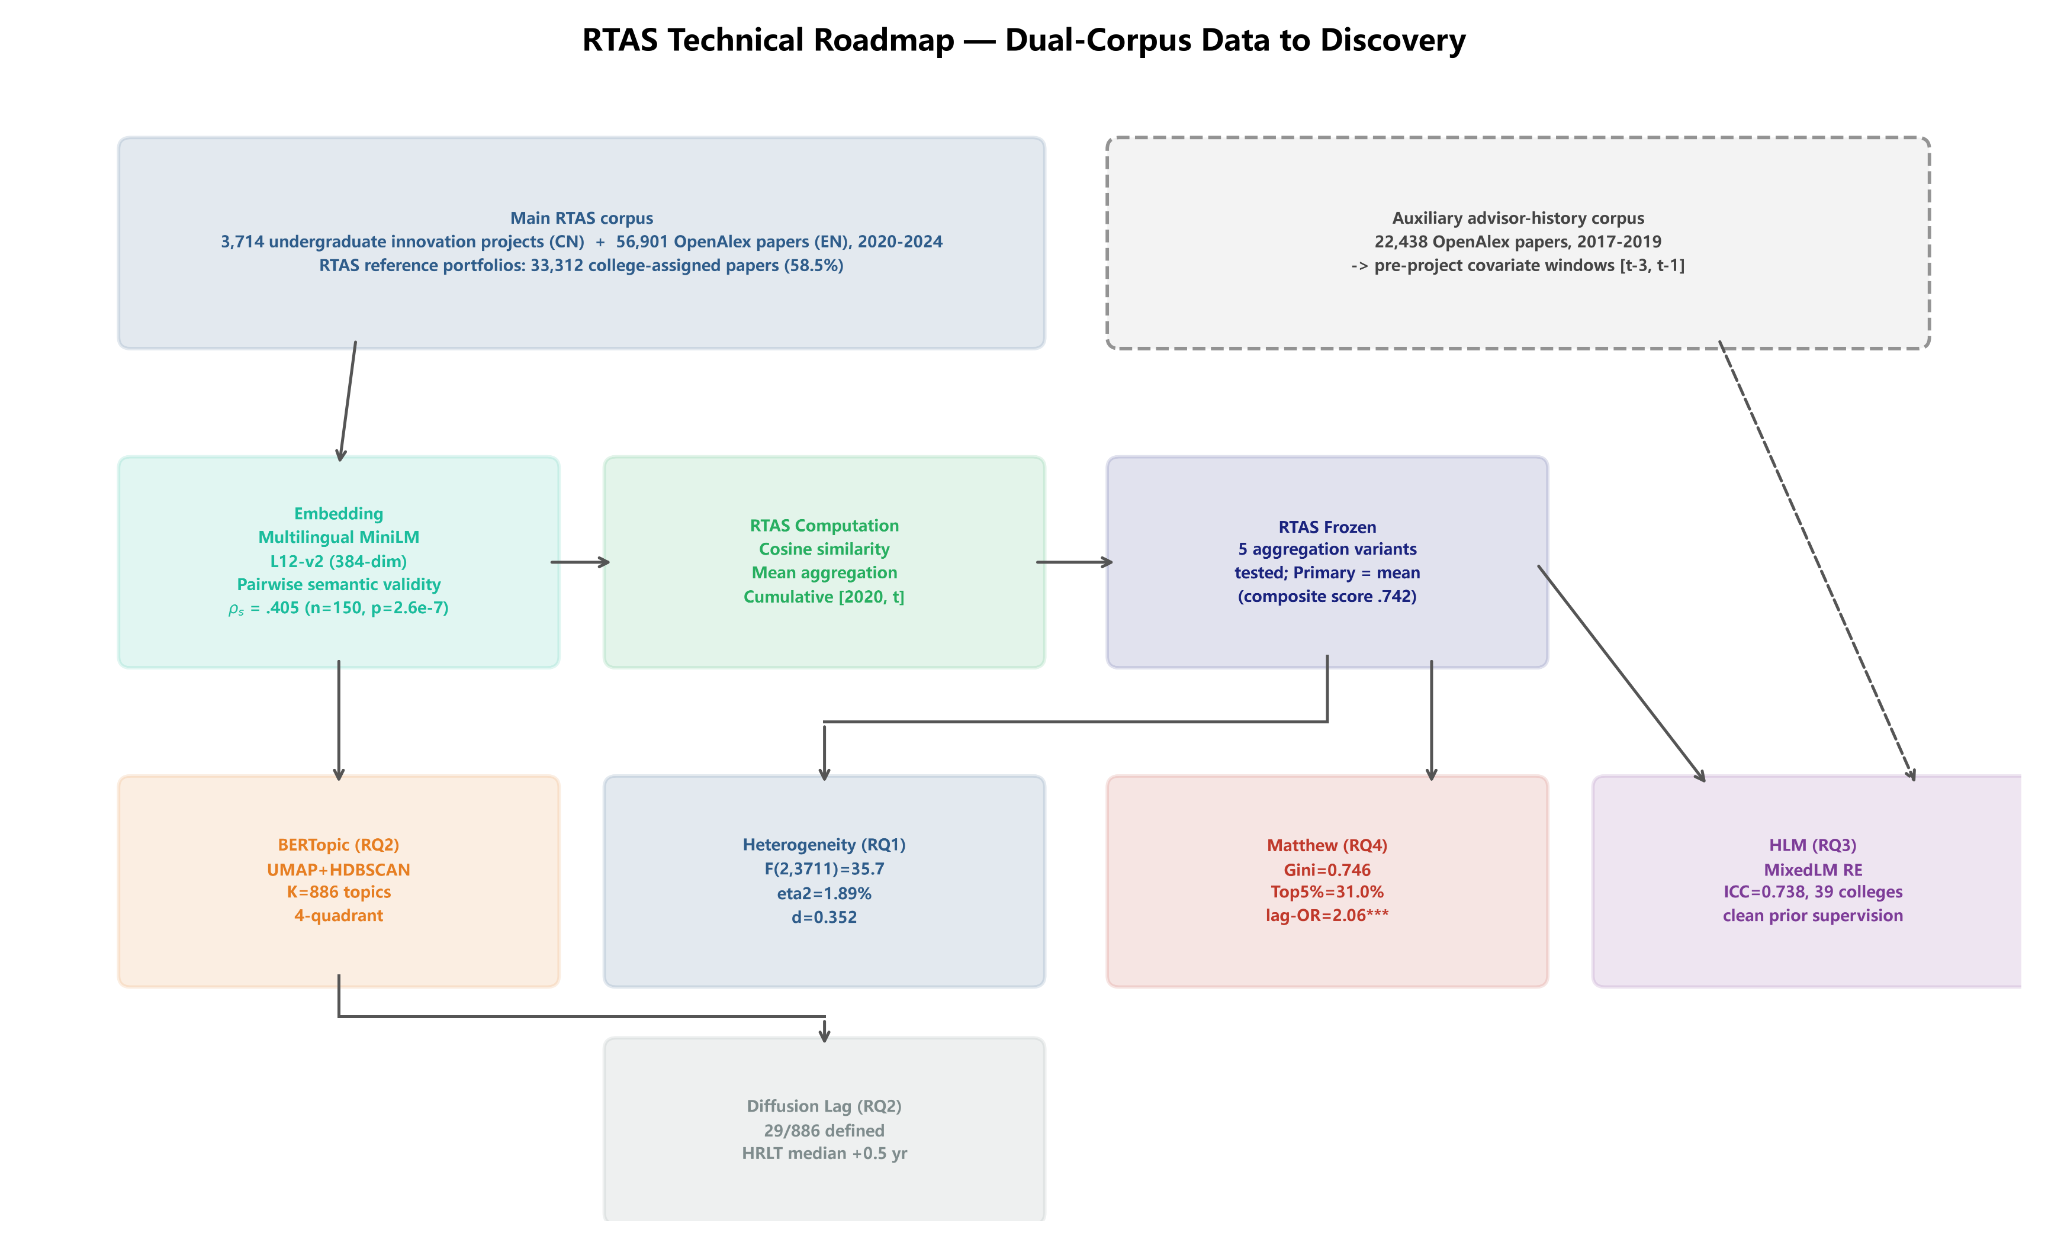
\includegraphics[width=0.98\linewidth]{Figure1_Roadmap.png}
\caption{Analytical roadmap and data structure. The 2020--2024 retrieval corpus contains 56,901 OpenAlex articles and 3,714 undergraduate innovation projects. Of the article corpus, 33,312 articles (58.5\%) receive at least one college assignment through advisor--author matching and form the college-specific RTAS reference portfolios. The full 56,901-article corpus is combined with all project titles for BERTopic. The auxiliary 2017--2019 OpenAlex pool is used only for temporally prior advisor covariates.}
\label{fig:roadmap}
\end{figure}

\section{Data and Methods}

\subsection{Data sources and corpus tiers}

\textbf{Projects.} The project corpus contains 3,714 undergraduate innovation projects approved at Wuhan University in 2020--2024: 1,375 university-level (37.0\%), 1,657 provincial-level (44.6\%), and 682 national-level (18.4\%). The project records were compiled from administrative records supplied by teaching administrators in the 40 colleges and subsequently consolidated into a unified study dataset. Each record contains title (project titles contain 92.3\% Chinese characters on average), level, year, college (40), and advisor information. Using the same delimiter and normalization rules as the advisor-covariate construction, multi-advisor fields were split into individual advisors: 1,834 individual advisors and 4,244 distinct advisor--project links are represented, and 528 projects are co-supervised. We additionally re-parsed the four official approval lists for 2021--2024, which carry a project-type field absent from the consolidated table: this independently reproduced the tier counts and the 1,834/4,244/528 advisor rebuild, and showed that the analytic sample pools two program tracks---158 unique projects (4.3\%; 74, 23, 26, and 35 in 2021--2024) are entrepreneurship training or practice projects rather than innovation training projects. No type-labeled official list exists for 2020, so track membership cannot be recovered for that cohort; a sensitivity analysis excluding the 158 identifiable entrepreneurship projects leaves every mixed-model conclusion unchanged (Online Resource 1, Table~S1). The archived 2022 official list itself contains no university-level entries, so that year's tier composition reflects source-registry coverage rather than any analytical reclassification.

\textbf{Articles.} A total of 56,901 OpenAlex records of type \texttt{article} were retrieved for Wuhan University (OpenAlex institution ID I37461747) for publication years 2020--2024 via cursor pagination on September 3, 2026. Titles were predominantly English: 56,858 of 56,901 titles (99.9\%) contained no Chinese characters; yearly counts were 9,970 / 10,117 / 12,002 / 11,954 / 12,858. OpenAlex provides an open scholarly metadata infrastructure \citep{priem2022openalex}; recent comparative work documents strong reference coverage while also identifying database-specific limitations \citep{culbert2025openalex}. An additional 22,438 articles published in 2017--2019 were retrieved on September 4, 2026 (total 79,339) and serve \emph{only} to compute advisors' pre-project publication windows; these records do not enter RTAS or topic modeling.

\textbf{Advisor--article linkage.} Advisor names are converted to pinyin keys (forward and reverse), matched against normalized OpenAlex author names with a college prior; ambiguous keys are skipped. A total of 33,312 articles (58.5\%) are assigned to colleges (mean 1.37 colleges per matched article). Per project, advisor covariate status is matched (2,750), ambiguous (748), or unmatched (216), with unmatched covariates coded NA rather than zero.

\textbf{Three corpus tiers.} These are not interchangeable: (i) the retrieval corpus contains 56,901 articles and supplies the full denominator for article-side topic prevalence; (ii) the advisor-matched college portfolios contain 33,312 articles and are the only papers entering RTAS reference portfolios $P_{c,t}$; and (iii) the joint BERTopic corpus contains 60,615 documents = 56,901 article titles + 3,714 project titles.

\subsection{RTAS definition}

For college $c$, year $t$, and project $p$:
\begin{equation}
\mathrm{RTAS}(p,c,t)=
\frac{1}{|P_{c,t}|}
\sum_{j\in P_{c,t}}
\cos(\mathbf e_p,\mathbf e_j),
\end{equation}
where $\mathbf e_p$ is the L2-normalized 384-dimensional embedding of the project title, and $P_{c,t}$ is the set of unique articles assigned to college $c$ over the cumulative window $[2020,t]$ via advisor--author linkage. If an article is linked to multiple advisors within the same college, it is counted once in that college portfolio; if it is linked to advisors in multiple colleges, it is counted once per college. Aggregation is the mean cosine.

Titles are used because the original project records contain no additional unstructured text beyond the title, making titles the only symmetric, cross-lingually comparable text unit available on both sides. Although article abstracts are available for a subset of OpenAlex records, no corresponding project abstracts exist in the institutional records; using article abstracts would therefore introduce a systematic information-granularity asymmetry between the two corpora. The resulting semantic sparsity is discussed in Sect.~\ref{sec:limitations}. RTAS therefore operationalizes local research alignment using the \emph{observed advisor-linked college research portfolio}; it does not measure novelty or influence. No citation or journal-tier information enters the score, although advisor covariates use pre-project publication counts from the institution-linked OpenAlex corpus.

RTAS is distinct from scholar-level research--teaching composites such as the RT-score \citep{scafetta2025rt} and from correlational studies of research and teaching indicators \citep{maisano2023empirical}: it is a project-level semantic alignment measure and is not used for performance ranking.

\subsection{Embedding and aggregation choice}

Embeddings use \texttt{paraphrase-multilingual-MiniLM-L12-v2} (384-dimensional), a multilingual Sentence-BERT family model built on Siamese sentence embeddings and multilingual knowledge distillation \citep{reimers2019sbert,reimers2020multilingual}. The model was selected for Chinese--English coverage and computational efficiency on the 60,615-document corpus; embedding-level validity was evaluated separately below. Five aggregation variants (mean, top-5/10/20 mean, centroid) were evaluated on the earlier 12,000-article development pool under a pre-specified composite rule. The normalized composite weighted known-groups separation ($\eta^2$ of a project-level analysis of variance [ANOVA]) by 0.45, temporal stability by 0.30, and topic-model K-stability by 0.25; a top-K variant would be preferred to the mean only if its composite score reached at least 95\% of the best score. Mean aggregation scored 0.742, while the best top-K comparator scored 0.480, so the mean was frozen as the primary RTAS and carried unchanged into the final 56,901-article corpus. Because funding-level separation contributed to this development-stage choice, the funding-level comparisons below are treated as descriptive rather than as independent validation. Frozen final-corpus RTAS descriptives are mean 0.1337, SD 0.0723, median 0.1362, range $[-0.0575,0.3960]$, $N=3,714$. Table~\ref{tab:selection} summarizes the frozen aggregation-selection decision.

\begin{table}[H]
\centering
\caption{Primary RTAS aggregation-selection summary.}
\label{tab:selection}
\begin{threeparttable}
\begin{tabular}{lrl}
\toprule
Aggregation variant & Development-stage composite & Status\\
\midrule
Mean & \textbf{0.742} & \textbf{Primary (selected)}\\
Top-5 mean & 0.480 & Best top-K comparator\\
Top-10 mean & 0.447 & Not selected\\
Top-20 mean & 0.398 & Not selected\\
Centroid & 0.300 & Not selected\\
\bottomrule
\end{tabular}
\begin{tablenotes}\footnotesize
\item Composite scores are the frozen values from the earlier 12,000-article development pool and were not re-tuned after expansion to 56,901 articles. The selected mean aggregation was carried unchanged into the final corpus. The final-sample funding-level effect, $\eta^2=0.0189$ (1.89\%), is reported separately in Sect.~3.1 and should not be confused with development-stage selection metrics.
\end{tablenotes}
\end{threeparttable}
\end{table}

\subsection{Validity program}

The primary validation protocols below were specified before execution and did not alter the frozen RTAS estimates. The BGE-M3 comparison was added post-freeze as an encoder robustness benchmark and likewise did not alter the primary RTAS pipeline.

\begin{itemize}
\item \textbf{Pairwise semantic validity (C1, embedding level).} The frozen validation set contains 150 randomly paired project-title--article-title pairs scored by a reference rater on a 1--4 relatedness rubric; 134/150 received score 1, so class imbalance is reported explicitly. Embedding cosine correlates with human relatedness at $\rho=0.405$ ($p=2.6\times10^{-7}$); a 10,000-resample bootstrap (seed 42) gives a 95\% confidence interval (CI) [0.281, 0.509], with permutation $p<.001$, Kendall $\tau_b=0.327$, and leave-one-out max $|\Delta\rho|=0.018$. Binary discrimination of related ($\ge2$) versus unrelated (=1) gives an area under the receiver operating characteristic curve (AUC) of 0.880 [0.793, 0.949]. C1 is evidence of pairwise semantic validity, not a completed construct-validity certification; the related-only subset ($n=16$) spans a restricted score range and is too small for stable within-stratum correlation estimation. Its $\rho=-0.253$ is reported for transparency and is not used for inference.

\item \textbf{Inter-rater reliability.} Ordinal agreement was summarized using quadratic-weighted Cohen's $\kappa$ \citep{cohen1968weighted}. Two independent human raters, blind to the reference scores and embedding values, scored a 50-pair subset: Rater A vs reference $\kappa=0.465$ (exact agreement 72\%); Rater B vs reference $\kappa=0.606$ (78\%; the reference rater's 46/50 ties at score 1 destabilize Spearman, so $\kappa$ and agreement are interpreted); A--B $\kappa=0.826$, $\rho=0.821$, agreement 90\%.

\item \textbf{Test--retest.} The same reference rater scored 40 reordered pairs after an approximately 12-day washout: $\kappa=0.643$, $\rho=0.688$ ($p<.001$), agreement 95\%.

\item \textbf{LLM second rater.} The API model alias \texttt{deepseek-reasoner} (temperature 0, prompt v1.1) rated all 150 pairs blind: $\kappa=0.459$, $\rho=0.638$ ($p=1.7\times10^{-18}$), agreement 93.3\%. Triangulation against Rater B yielded $\rho=0.621$ and AUC $=0.932$; these results are treated as converging evidence and do not replace the frozen C1 estimates.

\item \textbf{Naive lexical baselines.} Character 3--5-gram term frequency--inverse document frequency (TF--IDF) cosine, character 3-gram Jaccard, and BM25 Okapi \citep{robertson2009bm25} were applied directly to the Chinese--English pairs (cf. \citealp{hamers1989similarity} for cosine/Jaccard similarity in scientometric research). Applied without translation alignment, these direct lexical baselines yielded $\rho=0.296$--$0.300$ and AUC $=0.637$--$0.638$ (TF--IDF: $\rho=0.300$, AUC $=0.638$; Jaccard: $\rho=0.296$, AUC $=0.637$; BM25: $\rho=0.298$, AUC $=0.637$), below MiniLM's 0.405 / 0.880. The comparison supports the use of the multilingual semantic encoder over these direct lexical-overlap baselines; it makes no claim against translation-based or stronger cross-lingual methods.

\item \textbf{Post-freeze BGE-M3 benchmark.} Re-encoding the same 150 reference-rated pairs with BGE-M3 \citep{chen2024m3embedding} yielded $\rho=0.334$ and AUC $=0.811$. In 2,000 paired bootstrap resamples (seed 42), the BGE-minus-MiniLM differences were $\Delta\rho=-0.071$ (95\% CI [$-0.187$, 0.036]) and $\Delta$AUC $=-0.069$ (95\% CI [$-0.179$, 0.032]). There was no evidence that BGE-M3 improved pairwise validity relative to the frozen MiniLM encoder, so MiniLM was retained as primary.
\end{itemize}

Table~\ref{tab:validity} summarizes the embedding-level validity and reliability checks.

\begin{table}[H]
\centering
\caption{Summary of RTAS embedding-level validity and reliability checks.}
\label{tab:validity}
\begin{tabular}{p{0.27\linewidth}p{0.18\linewidth}p{0.43\linewidth}}
\toprule
Check & Sample & Main result\\
\midrule
Pairwise semantic validity & 150 pairs & Spearman $\rho=0.405$; AUC $=0.880$ [0.793, 0.949]\\
Independent human raters & 50 pairs & Quadratic-weighted $\kappa=0.465/0.606$ vs reference; A--B $\kappa=0.826$\\
Test--retest & 40 pairs & $\kappa=0.643$; $\rho=0.688$; 95\% agreement\\
LLM second rater & 150 pairs & $\kappa=0.459$; $\rho=0.638$; 93.3\% agreement\\
Naive lexical baselines (TF--IDF/Jaccard/BM25) & 150 pairs & $\rho=0.296$--0.300; AUC $=0.637$--0.638\\
BGE-M3 robustness & 150 pairs & $\rho=0.334$; AUC $=0.811$; paired-bootstrap differences include 0\\
\bottomrule
\end{tabular}
\end{table}

\subsection{Topic modeling}

BERTopic \citep{grootendorst2022bertopic} was fit to the 60,615-document joint corpus using the same multilingual MiniLM embeddings. Frozen Uniform Manifold Approximation and Projection (UMAP) parameters were \texttt{n\_neighbors=15}, \texttt{n\_components=5}, \texttt{min\_dist=0.0}, cosine distance, and \texttt{random\_state=42} \citep{mcinnes2018umap}. Hierarchical Density-Based Spatial Clustering of Applications with Noise (HDBSCAN) used \texttt{min\_cluster\_size=10}, \texttt{min\_samples=5}, Euclidean distance in the UMAP space, and the EOM cluster-selection rule \citep{mcinnes2017hdbscan}; BERTopic used \texttt{top\_n\_words=10}, \texttt{n\_gram\_range=(1,2)}, multilingual mode, and class-based term frequency--inverse document frequency (c-TF-IDF) topic representation. HDBSCAN yielded 886 non-outlier topics plus 23,318 outlier documents (38.47\%), leaving 37,297 clustered documents (61.53\%). Quadrant and lag analyses are conditional on these 886 clustered topics. Across clustering-parameter sensitivity settings (minimum cluster size/minimum samples = 15/7, 20/10, 8/3), outlier rates remained stable (0.364--0.396) and the qualitative quadrant structure remained unchanged; topic counts varied with granularity (454--1,287), as expected.

\subsection{Analysis windows}

Each analysis uses the window its question requires. RTAS uses the cumulative window $[2020,t]$; advisor covariates use the pre-project window $[t-3,t-1]$ with year $<t$; diffusion lags use an annual first non-trivial presence rule. On the article side, a topic must reach at least three articles and at least 0.2\% of that year's articles (approximately 20--26 articles/year over 2020--2024). On the project side, it must reach at least two projects and at least 0.2\% of that year's projects.

\subsection{Statistical models}

\begin{itemize}
\item \textbf{RQ1.} One-way ANOVA with Tukey honestly significant difference (HSD) tests was used for familywise-adjusted pairwise comparisons ($\Delta=$ higher $-$ lower level). For the largest contrast (national vs university), a Welch unequal-variance $t$ test and Cohen's $d$ are reported as descriptive robustness summaries. The 95\% CI for $\eta^2$ was estimated by 10,000 bootstrap resamples (seed 42). These comparisons are descriptive, not confirmatory, because level separation contributed to aggregation selection.

\item \textbf{RQ2.} Quadrant classification followed prevalence thresholds pre-specified in the analysis protocol (article side: fixed $\ge1.5\%$; project side: fixed $\ge0.500\%$). If a fixed cutoff yielded fewer than two high-prevalence topics, the pre-specified fallback classified the top 20\% of topics on that side as high-prevalence. Under the frozen 886-topic solution, no topic reached the article-side 1.5\% cutoff (equivalent to approximately 854 of 56,901 articles), so the fallback was triggered. The resulting effective article-side cutoff was 0.0879\%, exactly 50 articles; because eight topics were tied at this cutoff (ranks 171--178), the inclusive $\ge$ rule classified 178 topics as high research-side prevalence. The project-side 0.500\% cutoff remained feasible, with 15 topics meeting the threshold, and was therefore retained. Article-side sensitivity was assessed using top-15\%, top-20\%, and top-25\% prevalence cutoffs. Diffusion lags are computed only for topics meeting the annual rule on both sides.

\item \textbf{RQ3.} Following standard multilevel modeling practice \citep{snijders2012multilevel}, a two-level random-intercept mixed model was estimated by restricted maximum likelihood (REML) in \texttt{statsmodels MixedLM} \citep{seabold2010statsmodels}, with projects nested within colleges (primary complete cases $n=3,231$, 39 colleges; high-confidence-match sensitivity $n=2,750$). Year was entered as a continuous variable centered at 2022. Fixed effects included provincial- and national-level indicators, log-transformed advisor pre-project three-year publication counts within the institution-linked OpenAlex corpus, and log-transformed prior supervisory load, defined as cumulative supervised projects in the observed registry with year $<$ the focal year (mean across co-advisors). Because the registry begins in 2020, this supervision-history covariate is left-censored at 2020. An unconditional means model gives the null intraclass correlation coefficient (ICC). Model fit is summarized using marginal $R^2$ (variance explained by the fixed effects) and conditional $R^2$ (variance explained jointly by fixed and random effects), following \citet{nakagawa2017r2}. For descriptive context, a separate one-way college ANOVA was calculated across the 39 colleges with at least two projects; the single-project college was retained only in descriptive summaries. As a post-freeze sensitivity, RTAS was recomputed after removing from each project's college reference portfolio all articles authored by any focal advisor, and the same mixed-model specification was re-estimated. Advisor-level dependence was examined separately on single-advisor projects: after complete-case restriction, college fixed effects were combined with advisor-clustered standard errors, and the clustering was repeated using college $\times$ normalized-advisor-name identifiers as a homonym guard. A crossed college--advisor random-intercept model was also examined diagnostically but converged to a boundary solution and was not used for substantive inference.

\item \textbf{RQ4.} Multi-advisor project fields were split using the same delimiter and normalization rules as the advisor-covariate construction, yielding 4,244 distinct advisor--project links across 1,834 individual advisors. National-project concentration is summarized using Gini and Pareto measures at this individual-advisor level. An advisor-year lagged logistic model estimates $P(\mathrm{nat}_t)$ from $\mathrm{nat}_{t-1}$, $\log(1+\mathrm{load}_{t-1})$, and categorical year fixed effects (2021 as the reference year because the $t-1$ lag makes 2021 the earliest outcome year), with standard errors clustered by advisor. The primary risk set requires advisors to be active in both $t-1$ and $t$ (979 advisor-years / 627 advisors); the expanded robustness risk set includes advisors active at $t-1$ and codes no project activity at $t$ as no national project (2,469 / 1,560). This lagged design avoids the circularity of a cross-sectional top-5\% regression in which top-5\% membership is itself defined from cumulative national-project counts. Separately, each project was classified once as top-5\% exposed if at least one focal advisor belonged to the top 5\% of individual advisors ranked by cumulative national-project count; these projects were compared descriptively with the remainder using a Welch unequal-variance $t$ test and Cohen's $d$. This comparison is not treated as an independent causal or confirmatory test.
\end{itemize}

All reported statistics were generated from frozen analysis outputs; values are rounded for presentation. Seed 42 was used wherever stochastic procedures required a random seed. Analyses were conducted in Python 3.13; package dependencies are archived with the analysis code.

\section{Results}

\subsection{Funding level and alignment (RQ1)}

Mean RTAS rises monotonically with level: university 0.1212, provincial 0.1391, national 0.1460. ANOVA $F(2,3711)=35.72$, $p=4.3\times10^{-16}$, $\eta^2=1.89\%$ (95\% bootstrap CI [1.14\%, 2.86\%]). Tukey HSD: P--U $+0.0179$ ($p<0.001$), N--U $+0.0248$ ($p<0.001$), N--P $+0.0070$ ($p_{\mathrm{adj}}=0.082$, ns); the largest pairwise gap (N--U) has Welch $t=7.375$, $p=2.9\times10^{-13}$, $d=+0.352$. The mean ordering is University $<$ Provincial $<$ National, although the provincial--national contrast is not statistically significant. Figure~\ref{fig:funding} shows the project-level distributions and Tukey HSD comparisons. In the hierarchical model, however, provincial ($\beta=+0.0006$) and national ($\beta=-0.0016$) indicators are indistinguishable from zero (95\% CIs cross 0): the raw level differences are attenuated to near zero after accounting for college and advisor context; the adjusted funding-level coefficients are not statistically distinguishable from zero in this model.

\begin{figure}[H]
\centering
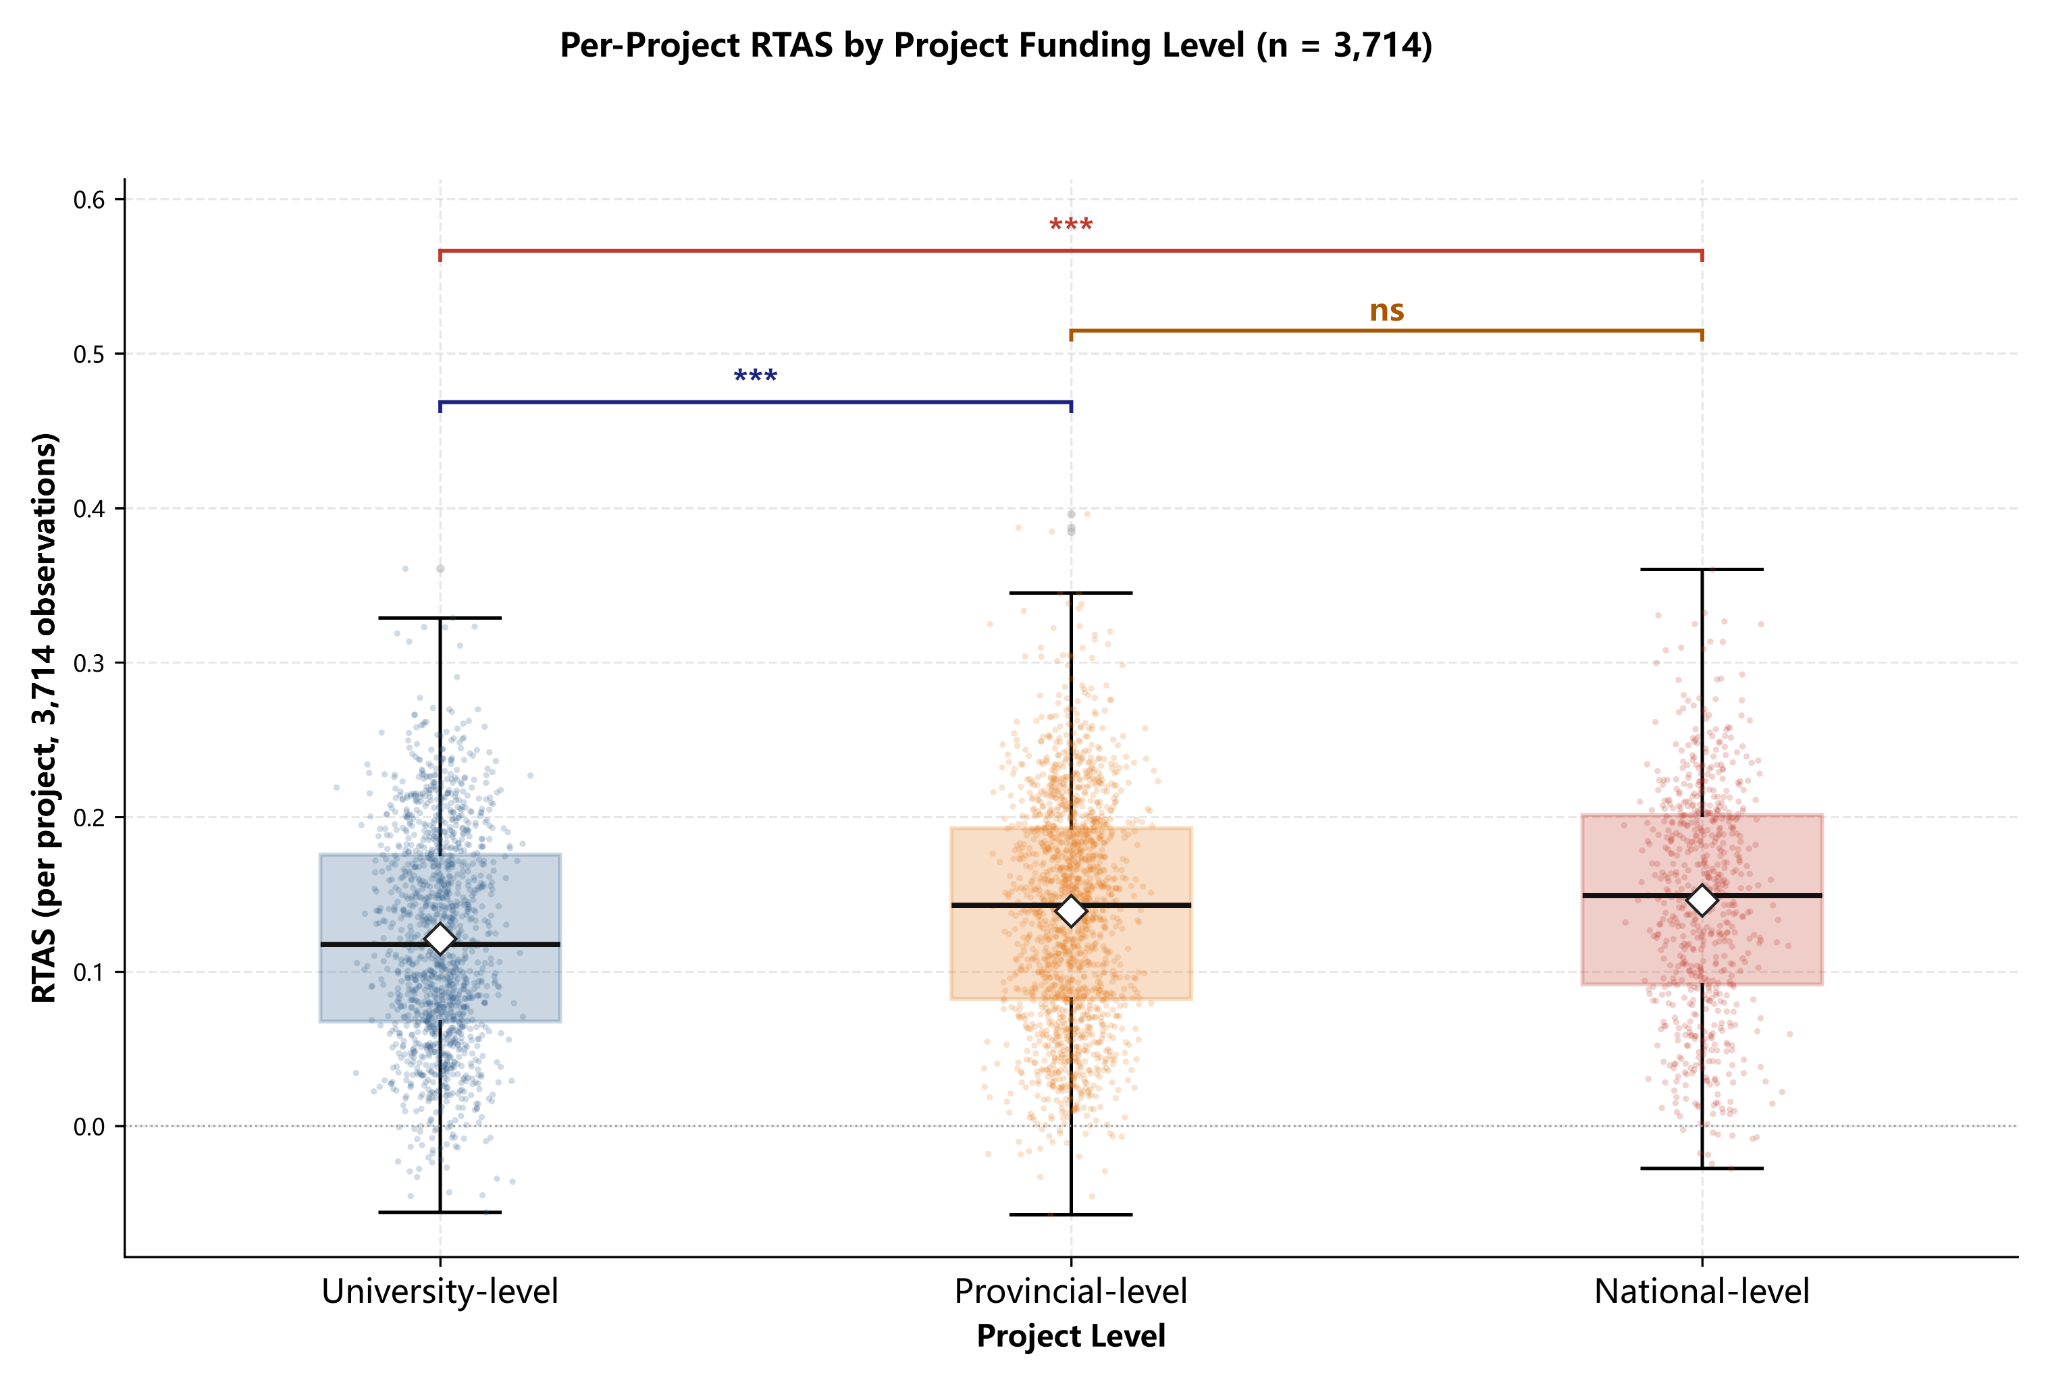
\includegraphics[width=0.94\linewidth]{Figure3_FundingLevel.png}
\caption{Project-level RTAS distributions by funding level. Boxes show the interquartile range with median lines, jittered points show individual projects, and diamonds show group means. Brackets report Tukey HSD familywise comparisons; *** denotes $p<.001$ and ns denotes not significant.}
\label{fig:funding}
\end{figure}

\subsection{Static prevalence quadrants (RQ2, classification)}

Classifying the 886 clustered topics by cumulative prevalence yields Table~\ref{tab:quadrants}. HRLT dominates the high-research region: 173 topics have high article-side but low project-side prevalence, forming the largest prevalence-asymmetry block. LRHT comprises only 10 topics. Threshold sensitivity (article-side top-15\%/20\%/25\%) leaves the qualitative pattern stable: HRLT 128/173/224, LRHT 10/10/8, HRHT 5/5/7, and all 29 lag-definable topics remain in HRLT/HRHT. Quadrant labels carry no temporal meaning; temporal interpretation is restricted to topics whose lags are defined. Figure~\ref{fig:quadrants} maps the frozen quadrant classification; additional count summaries and descriptive project-side topic dynamics are provided in the Supplementary Material (Online Resource 1).

\begin{table}[H]
\centering
\caption{Static topic-prevalence quadrants (pooled 2020--2024 prevalence).}
\label{tab:quadrants}
\begin{tabular}{lrrrl}
\toprule
Quadrant & Topics & Articles & Projects & Meaning\\
\midrule
HRHT & 5 & 2,090 & 308 & high research, high project\\
HRLT & 173 & 18,141 & 399 & high research, low project\\
LRHT & 10 & 219 & 278 & low research, high project\\
LRLT & 698 & 15,097 & 765 & low on both sides\\
\midrule
Total & 886 & 35,547 & 1,750 & clustered documents only\\
\bottomrule
\end{tabular}
\end{table}

\begin{figure}[H]
\centering
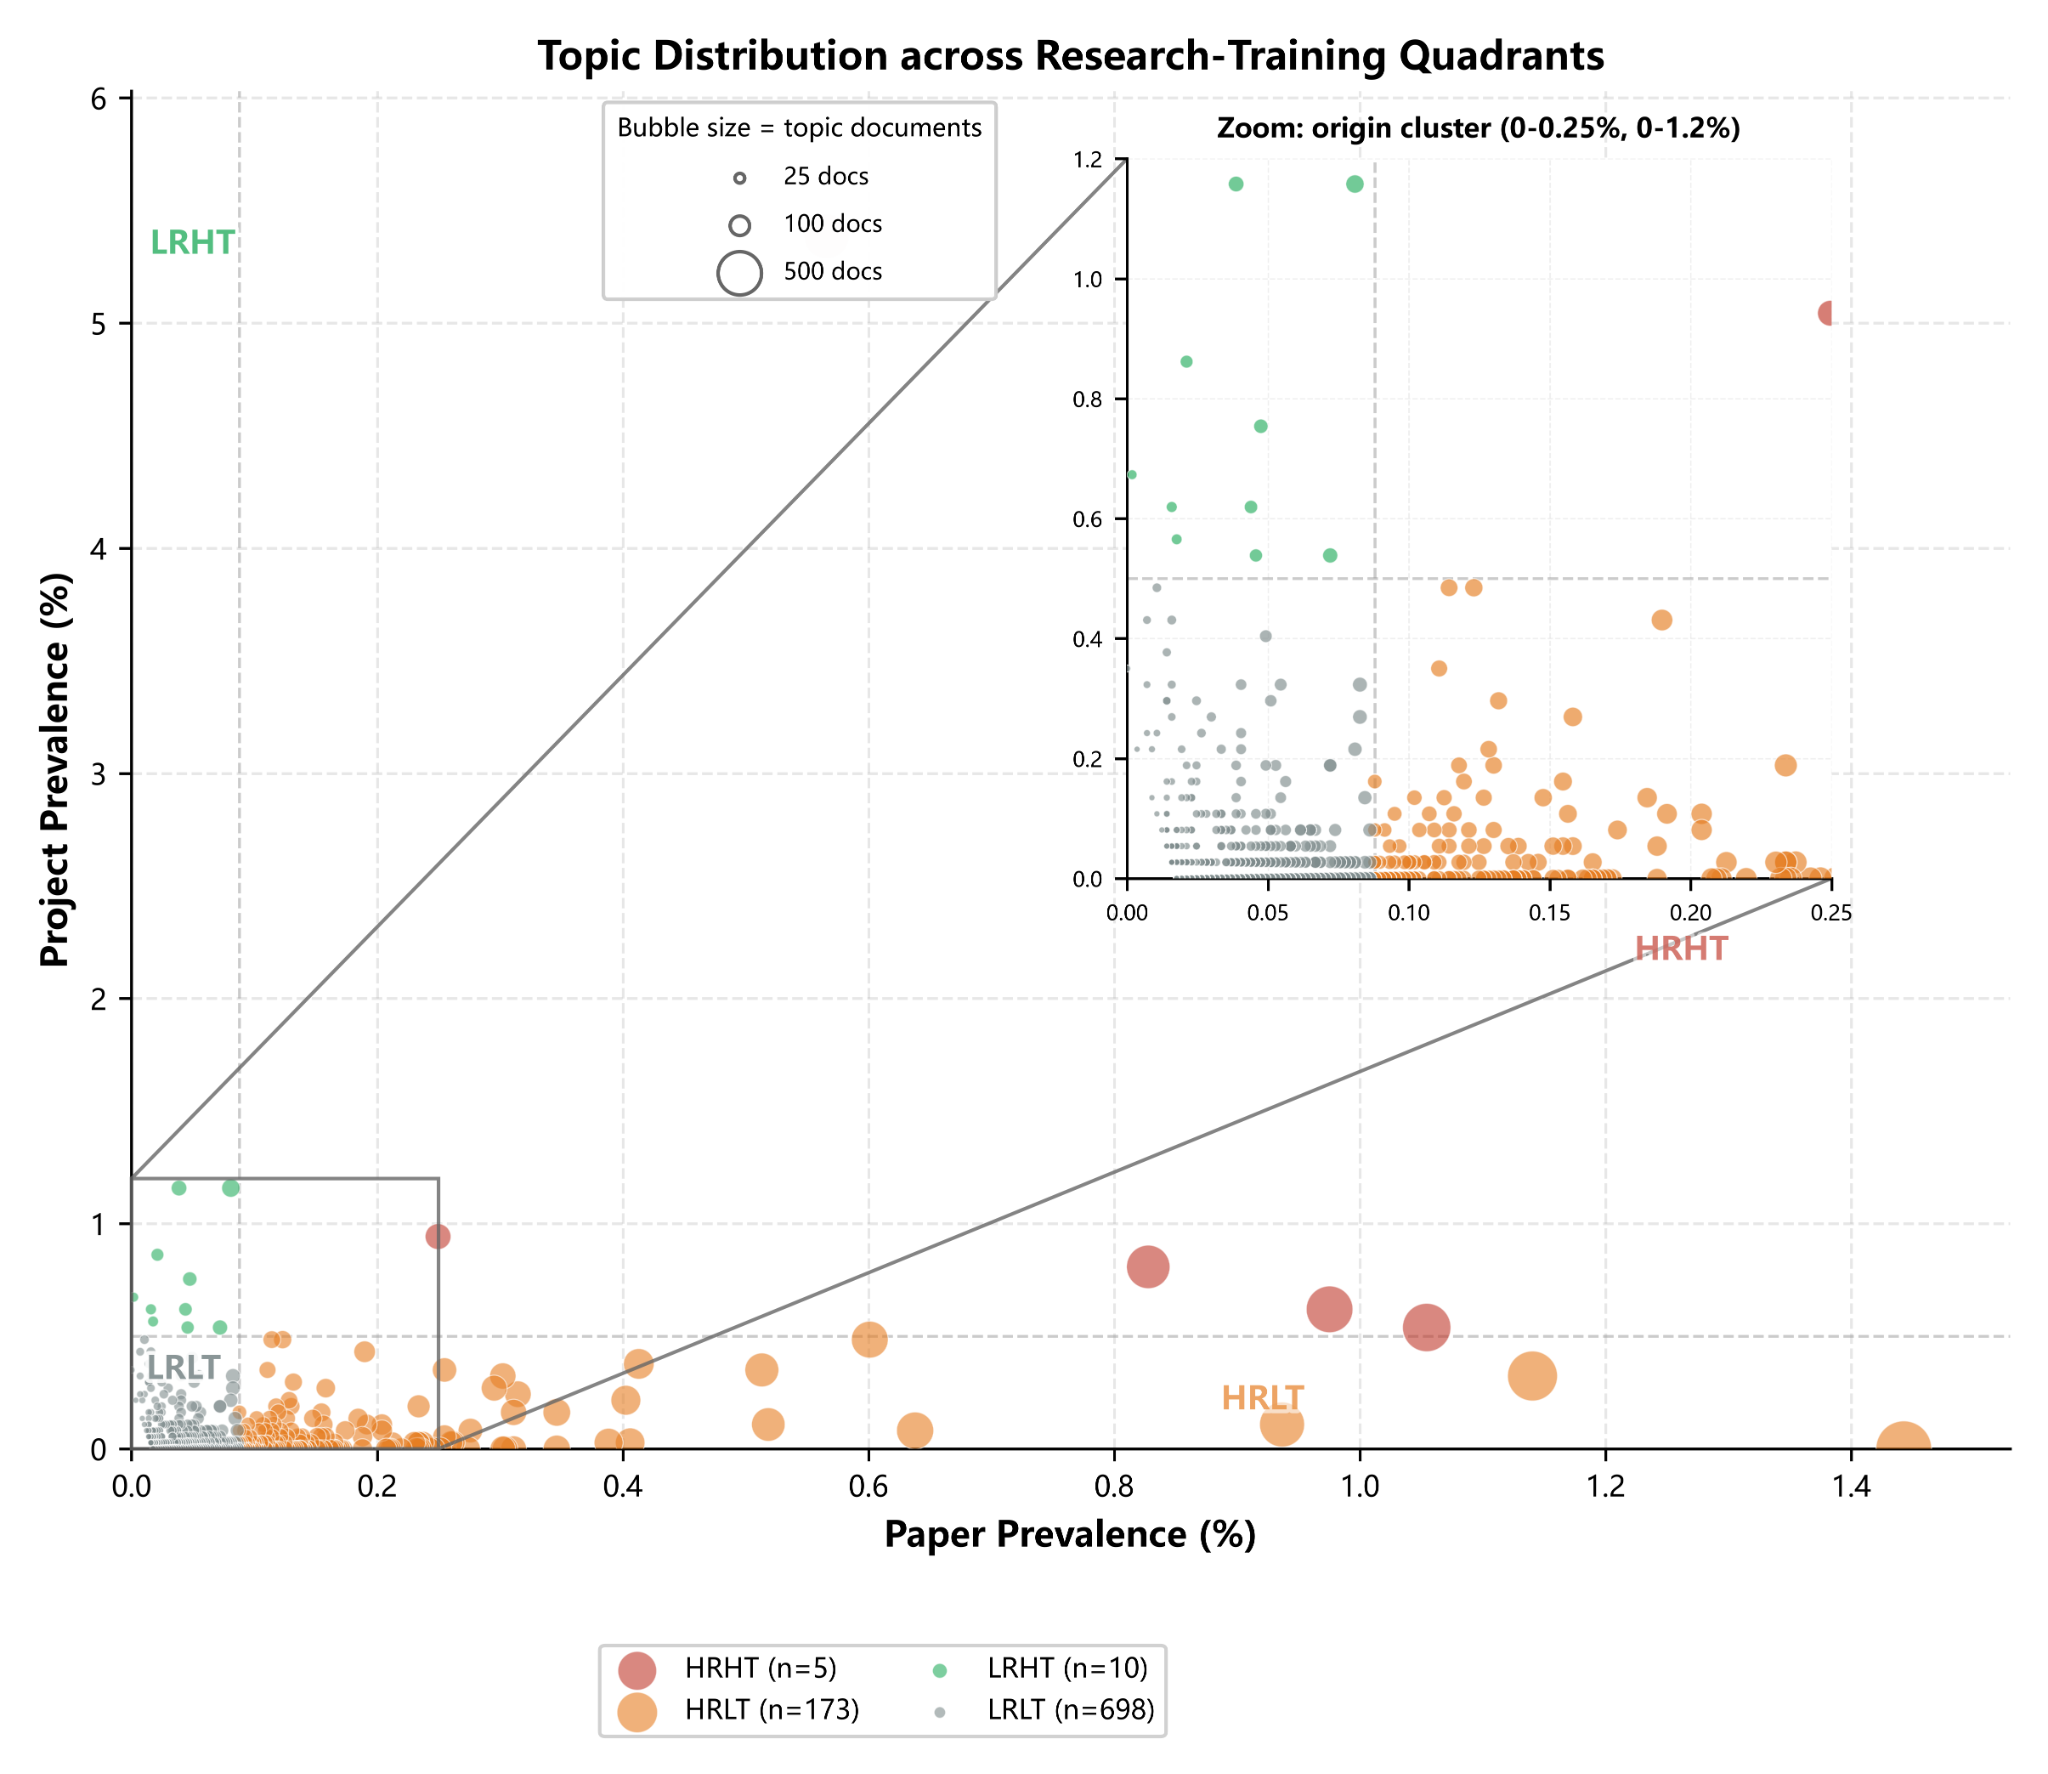
\includegraphics[width=0.98\linewidth]{Figure2_QuadrantScatter.png}
\caption{Static research--training topic prevalence across 886 non-outlier BERTopic topics. The horizontal axis shows article-side prevalence and the vertical axis project-side prevalence. Dashed lines indicate the frozen high/low thresholds. Bubble size reflects topic document count; the inset magnifies the dense low-prevalence region. Quadrant labels describe pooled prevalence only and carry no temporal interpretation.}
\label{fig:quadrants}
\end{figure}

\subsection{Diffusion lags where definable (RQ2, temporal)}

Under the annual first non-trivial presence rule, only 29 of 886 topics (3.27\%) are definable on both sides---24 in HRLT and five in HRHT. Overall median lag is 0 years (mean $+0.59$). In HRLT, the median lag is $+0.5$ years (mean $+0.79$): 50.0\% (12/24) of these topics show research-side presence first, 37.5\% show same-year first non-trivial presence, and 12.5\% show project-side presence first. LRHT (0/10) and LRLT (0/698) never reach the article-side annual threshold in any single year, so their lags are \emph{undefined in this corpus} rather than treated as missing. Consequently, statements that training content ``trails research'' cannot be made for these strata here; a curriculum-syllabus audit would provide a more appropriate source of evidence. Figure~\ref{fig:lags} displays the overall defined-lag distribution and the HRLT/HRHT comparison.

\begin{figure}[H]
\centering
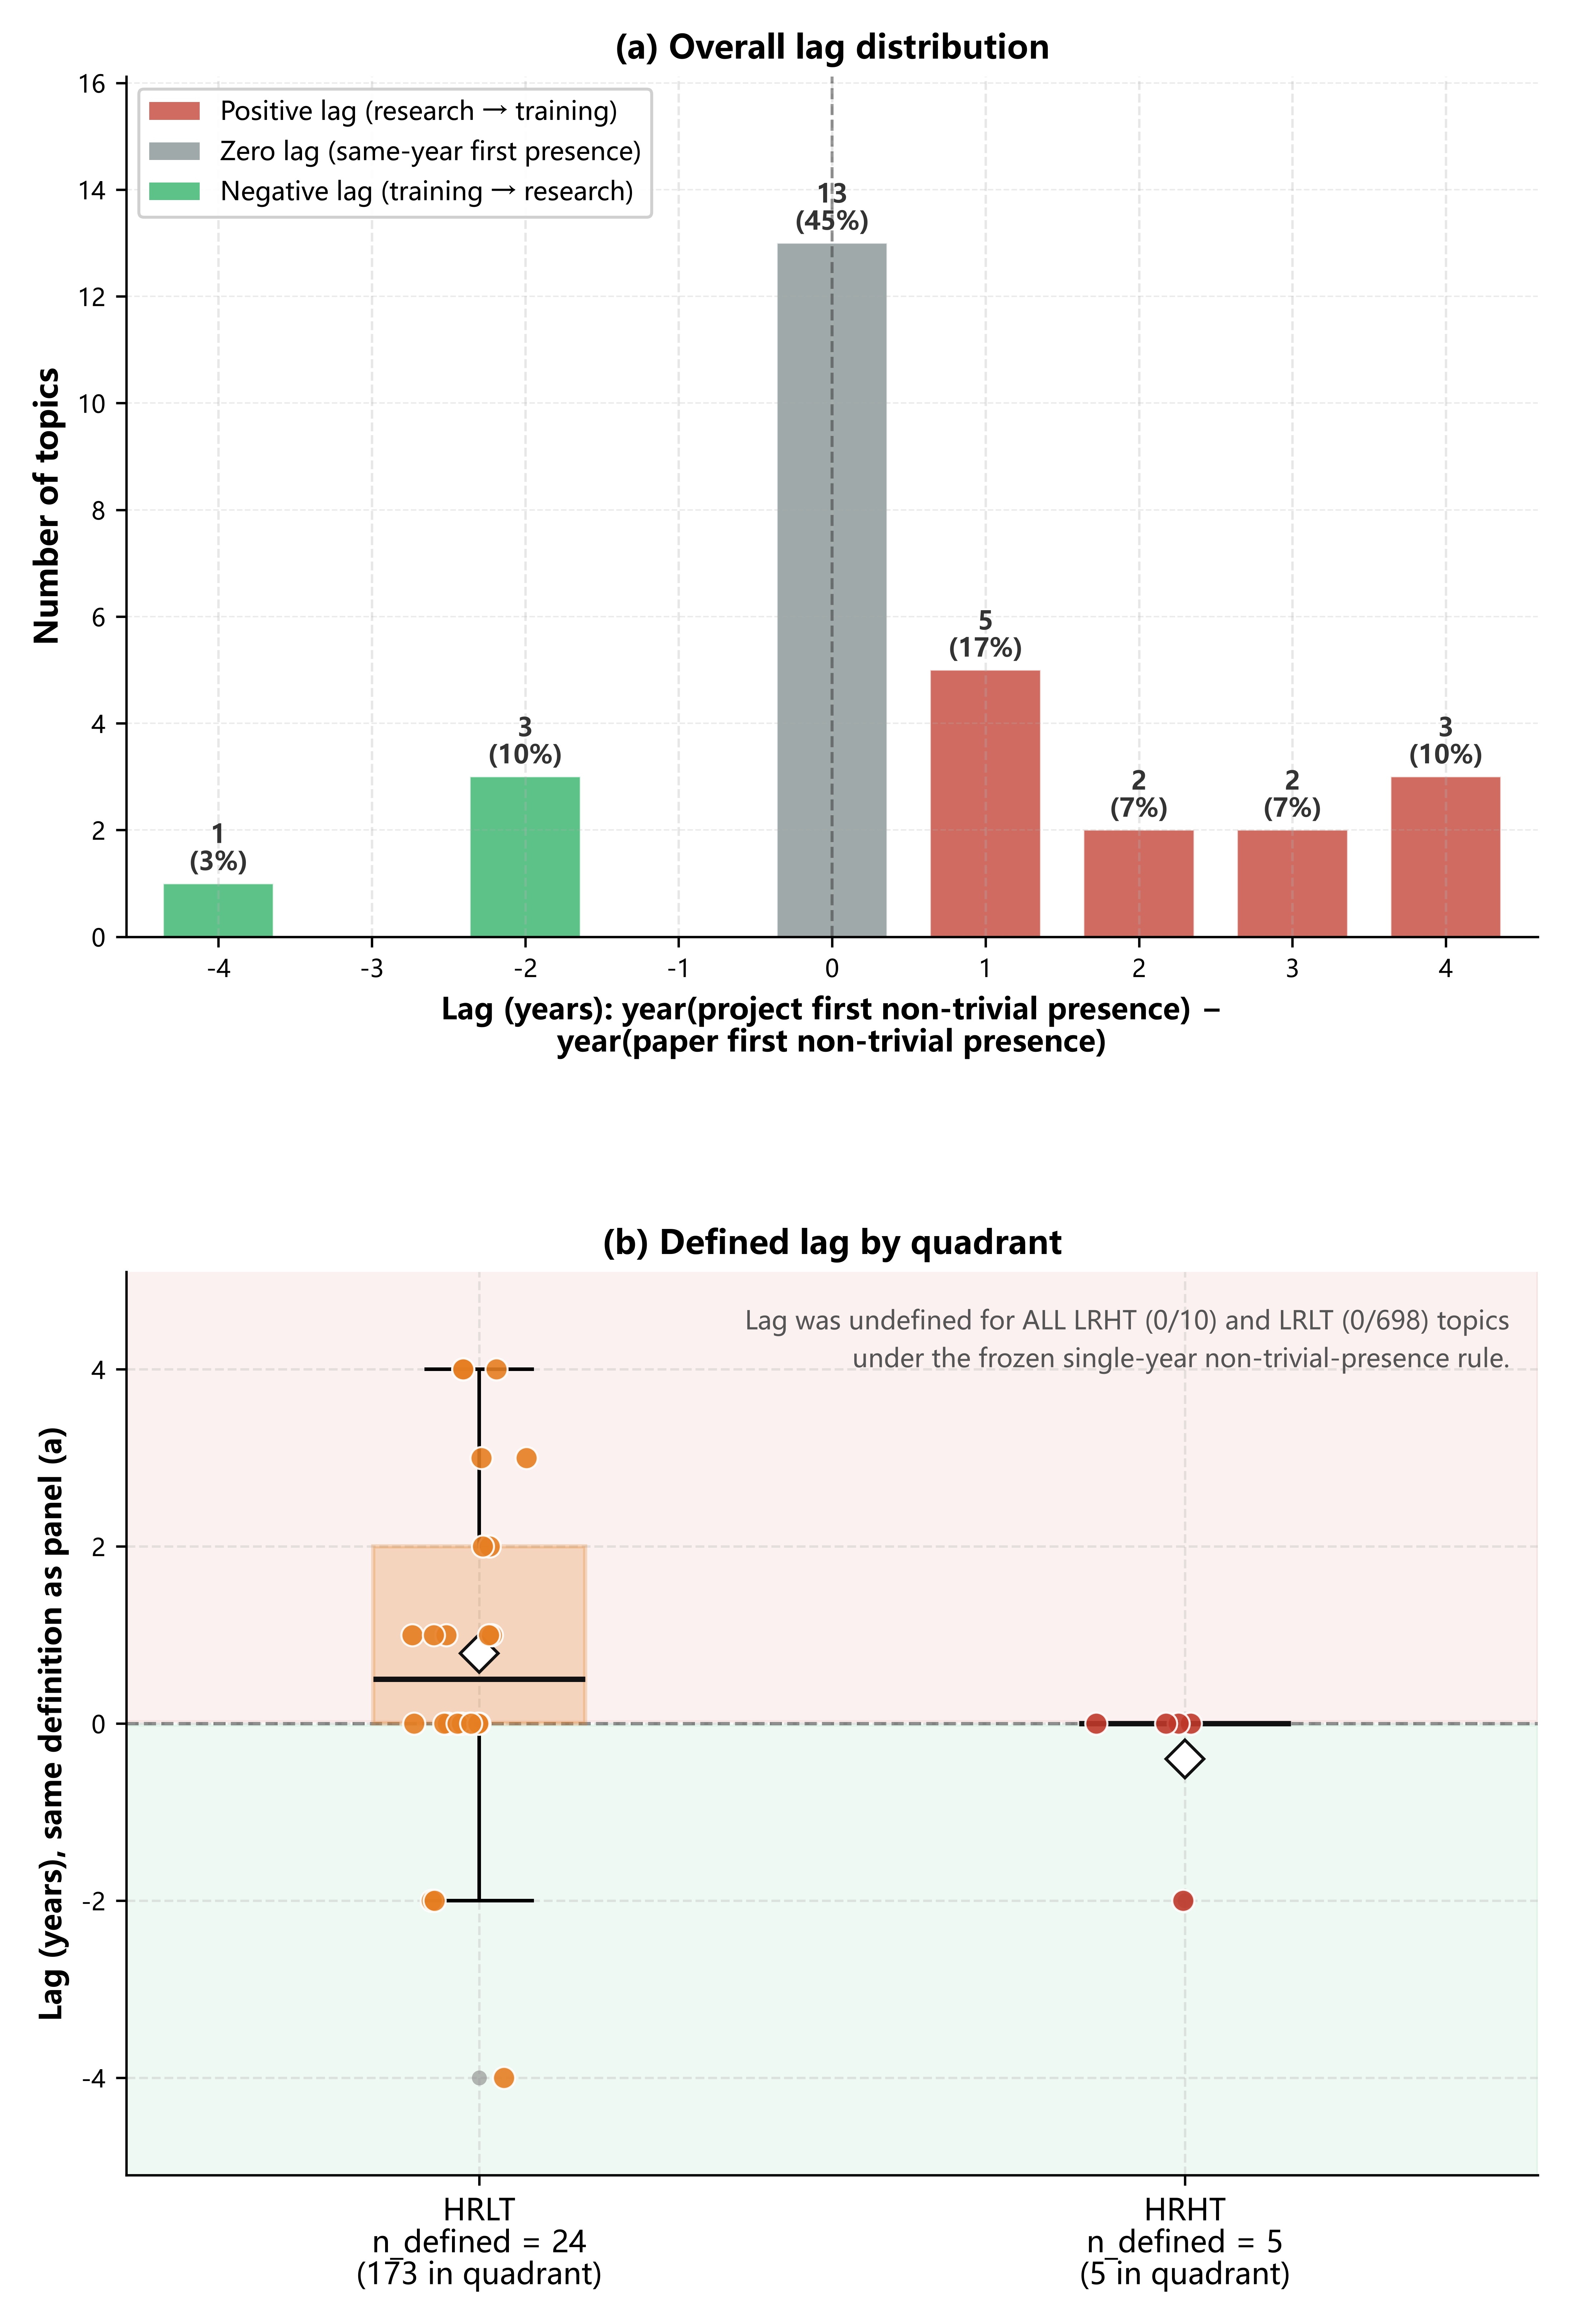
\includegraphics[height=0.78\textheight,keepaspectratio]{Figure4_DiffusionLag_Stacked.png}
\caption{Diffusion-lag patterns for topics whose first non-trivial annual presence is definable on both sides. Panel (a) shows the overall distribution of defined lags. Panel (b) compares HRLT and HRHT topics. Positive lag indicates research-side first non-trivial presence before the project side; zero indicates same-year first non-trivial presence; negative values indicate project-side first presence before the research side.}
\label{fig:lags}
\end{figure}

\subsection{College context and advisor associations (RQ3)}

The unconditional means model gives ICC $=0.7523$; the full random-intercept model yields ICC $=0.7376$---about three quarters of RTAS variance lies between colleges. The marginal $R^2$ was 0.0075, whereas the conditional $R^2$ was 0.7395 \citep{nakagawa2017r2}, indicating that the observed fixed effects explained relatively little variance compared with the substantial between-college component. A separate descriptive one-way college ANOVA across the 39 colleges with at least two projects yielded $F(38,3674)=195.45$, $p<.001$, $\eta^2=66.90\%$; this fixed-group effect-size estimate is a different estimand from the mixed-model ICC because the sample and adjustment structure differ. Raw means for all 40 colleges, including the single-project college excluded from the ANOVA, are provided in the Supplementary Material (Online Resource 1).

Among the observed project-level covariates, the advisor measures show the clearest associations. Advisors' \textbf{pre-project 3-year publication count within the institution-linked OpenAlex corpus} is positively associated with alignment ($\beta=+0.0043$, $p=3.3\times10^{-9}$); moving from 0 to 10 such publications corresponds to approximately $+0.010$ RTAS (approximately 0.14 SD). \textbf{Prior supervisory load} is negatively associated ($\beta=-0.0063$, $p=1.9\times10^{-5}$), a pattern compatible with a capacity-dilution interpretation. \textbf{Year}, entered continuously and centered at 2022, is positively associated with RTAS ($\beta=+0.00313$ per year, $p<0.001$); funding-level indicators are not statistically distinguishable from zero. Because RTAS uses cumulative $[2020,t]$ reference portfolios, later cohorts are compared against progressively larger and compositionally changing portfolios; the year coefficient therefore represents a temporal association under a changing reference set rather than independent temporal improvement.

\textbf{Leave-advisor-out sensitivity.} Because focal advisors' own publications enter their college's reference portfolio, the advisor-publication coefficient could be partly mechanical. RTAS was therefore recomputed after removing all articles authored by any focal advisor of each project, and the same mixed-model specification was re-estimated on the same 3,231 complete cases. The advisor-publication coefficient attenuated by approximately 10.5\% (from $\beta=+0.00427$ to $\beta=+0.00382$) but remained positive and statistically significant ($p=5.3\times10^{-7}$; 95\% CI [0.00233, 0.00531]). ICC (0.738) and conditional $R^2$ (0.739) were virtually unchanged. Of the 3,714 projects, 2,081 (56\%) had at least one advisor-authored article removed (mean 7.97 articles removed; mean portfolio reduction 4.1\%); no project's portfolio became empty. This attenuation is consistent with some contribution from mechanical self-overlap, but most of the observed association persisted under the leave-advisor-out construction.

\textbf{Advisor-dependence sensitivity.} The primary model accounts for project clustering within colleges but does not include a separate advisor random effect, although advisors can supervise repeated projects and 528 projects are co-supervised. To examine within-advisor dependence without duplicating co-supervised projects, the sensitivity was restricted to the 3,186 single-advisor projects (2,716 complete cases; 1,221 advisors, 680 with at least two projects). A crossed random-intercept model, $(1|\mathrm{college})+(1|\mathrm{advisor})$, converged to a boundary solution with college variance estimated at zero and was not used for substantive inference. The conservative alternative---college fixed effects with standard errors clustered by advisor---left the substantive conclusions unchanged: pre-project publications $\beta=+0.0043$ ($p=1.5\times10^{-5}$; 95\% CI [0.0023, 0.0062]), prior supervisory load $\beta=-0.0053$ ($p=0.004$; 95\% CI [$-0.0088$, $-0.0017$]), year $\beta=+0.0026$ ($p=0.001$), and funding-level coefficients not statistically distinguishable from zero. A homonym guard using college $\times$ normalized-advisor-name clusters yielded 1,333 clusters rather than 1,221 raw-name clusters and produced virtually identical standard errors and the same inferential conclusions. The substantive fixed-effect conclusions were therefore robust to advisor-clustered inference in the single-advisor subset.

All estimates are observational associations, not causal identification. The high-confidence-match sensitivity sample preserves every coefficient sign and significance classification. Table~\ref{tab:hlm} reports the primary fixed-effect estimates; Figure~\ref{fig:college} shows the model-adjusted college random effects, and Figure~\ref{fig:hlm} summarizes the fixed effects graphically. Because RTAS also responds to disciplinary specialization, portfolio breadth, and title-language conventions, college-level results are not interpreted as performance.

\begin{table}[H]
\centering
\caption{Two-level random-intercept mixed model predicting RTAS.}
\label{tab:hlm}
\begin{tabular}{lrrr}
\toprule
Predictor & $\beta$ & 95\% CI & $p$\\
\midrule
Provincial vs university & 0.00062 & [$-0.00275$, 0.00398] & 0.720\\
National vs university & $-0.00162$ & [$-0.00585$, 0.00261] & 0.452\\
Year (per year; centered 2022) & 0.00313 & [0.00187, 0.00439] & $<0.001$\\
Advisor prior 3y works, $\log(1+x)$ & 0.00427 & [0.00285, 0.00568] & $<0.001$\\
Advisor prior supervised projects, $\log(1+x)$ & $-0.00629$ & [$-0.00917$, $-0.00341$] & $<0.001$\\
\bottomrule
\end{tabular}

\vspace{1mm}
\footnotesize Primary complete-case sample: $N=3,231$ projects in 39 colleges; REML; random intercept by college; ICC $=0.7376$.
\end{table}

\begin{figure}[H]
\centering
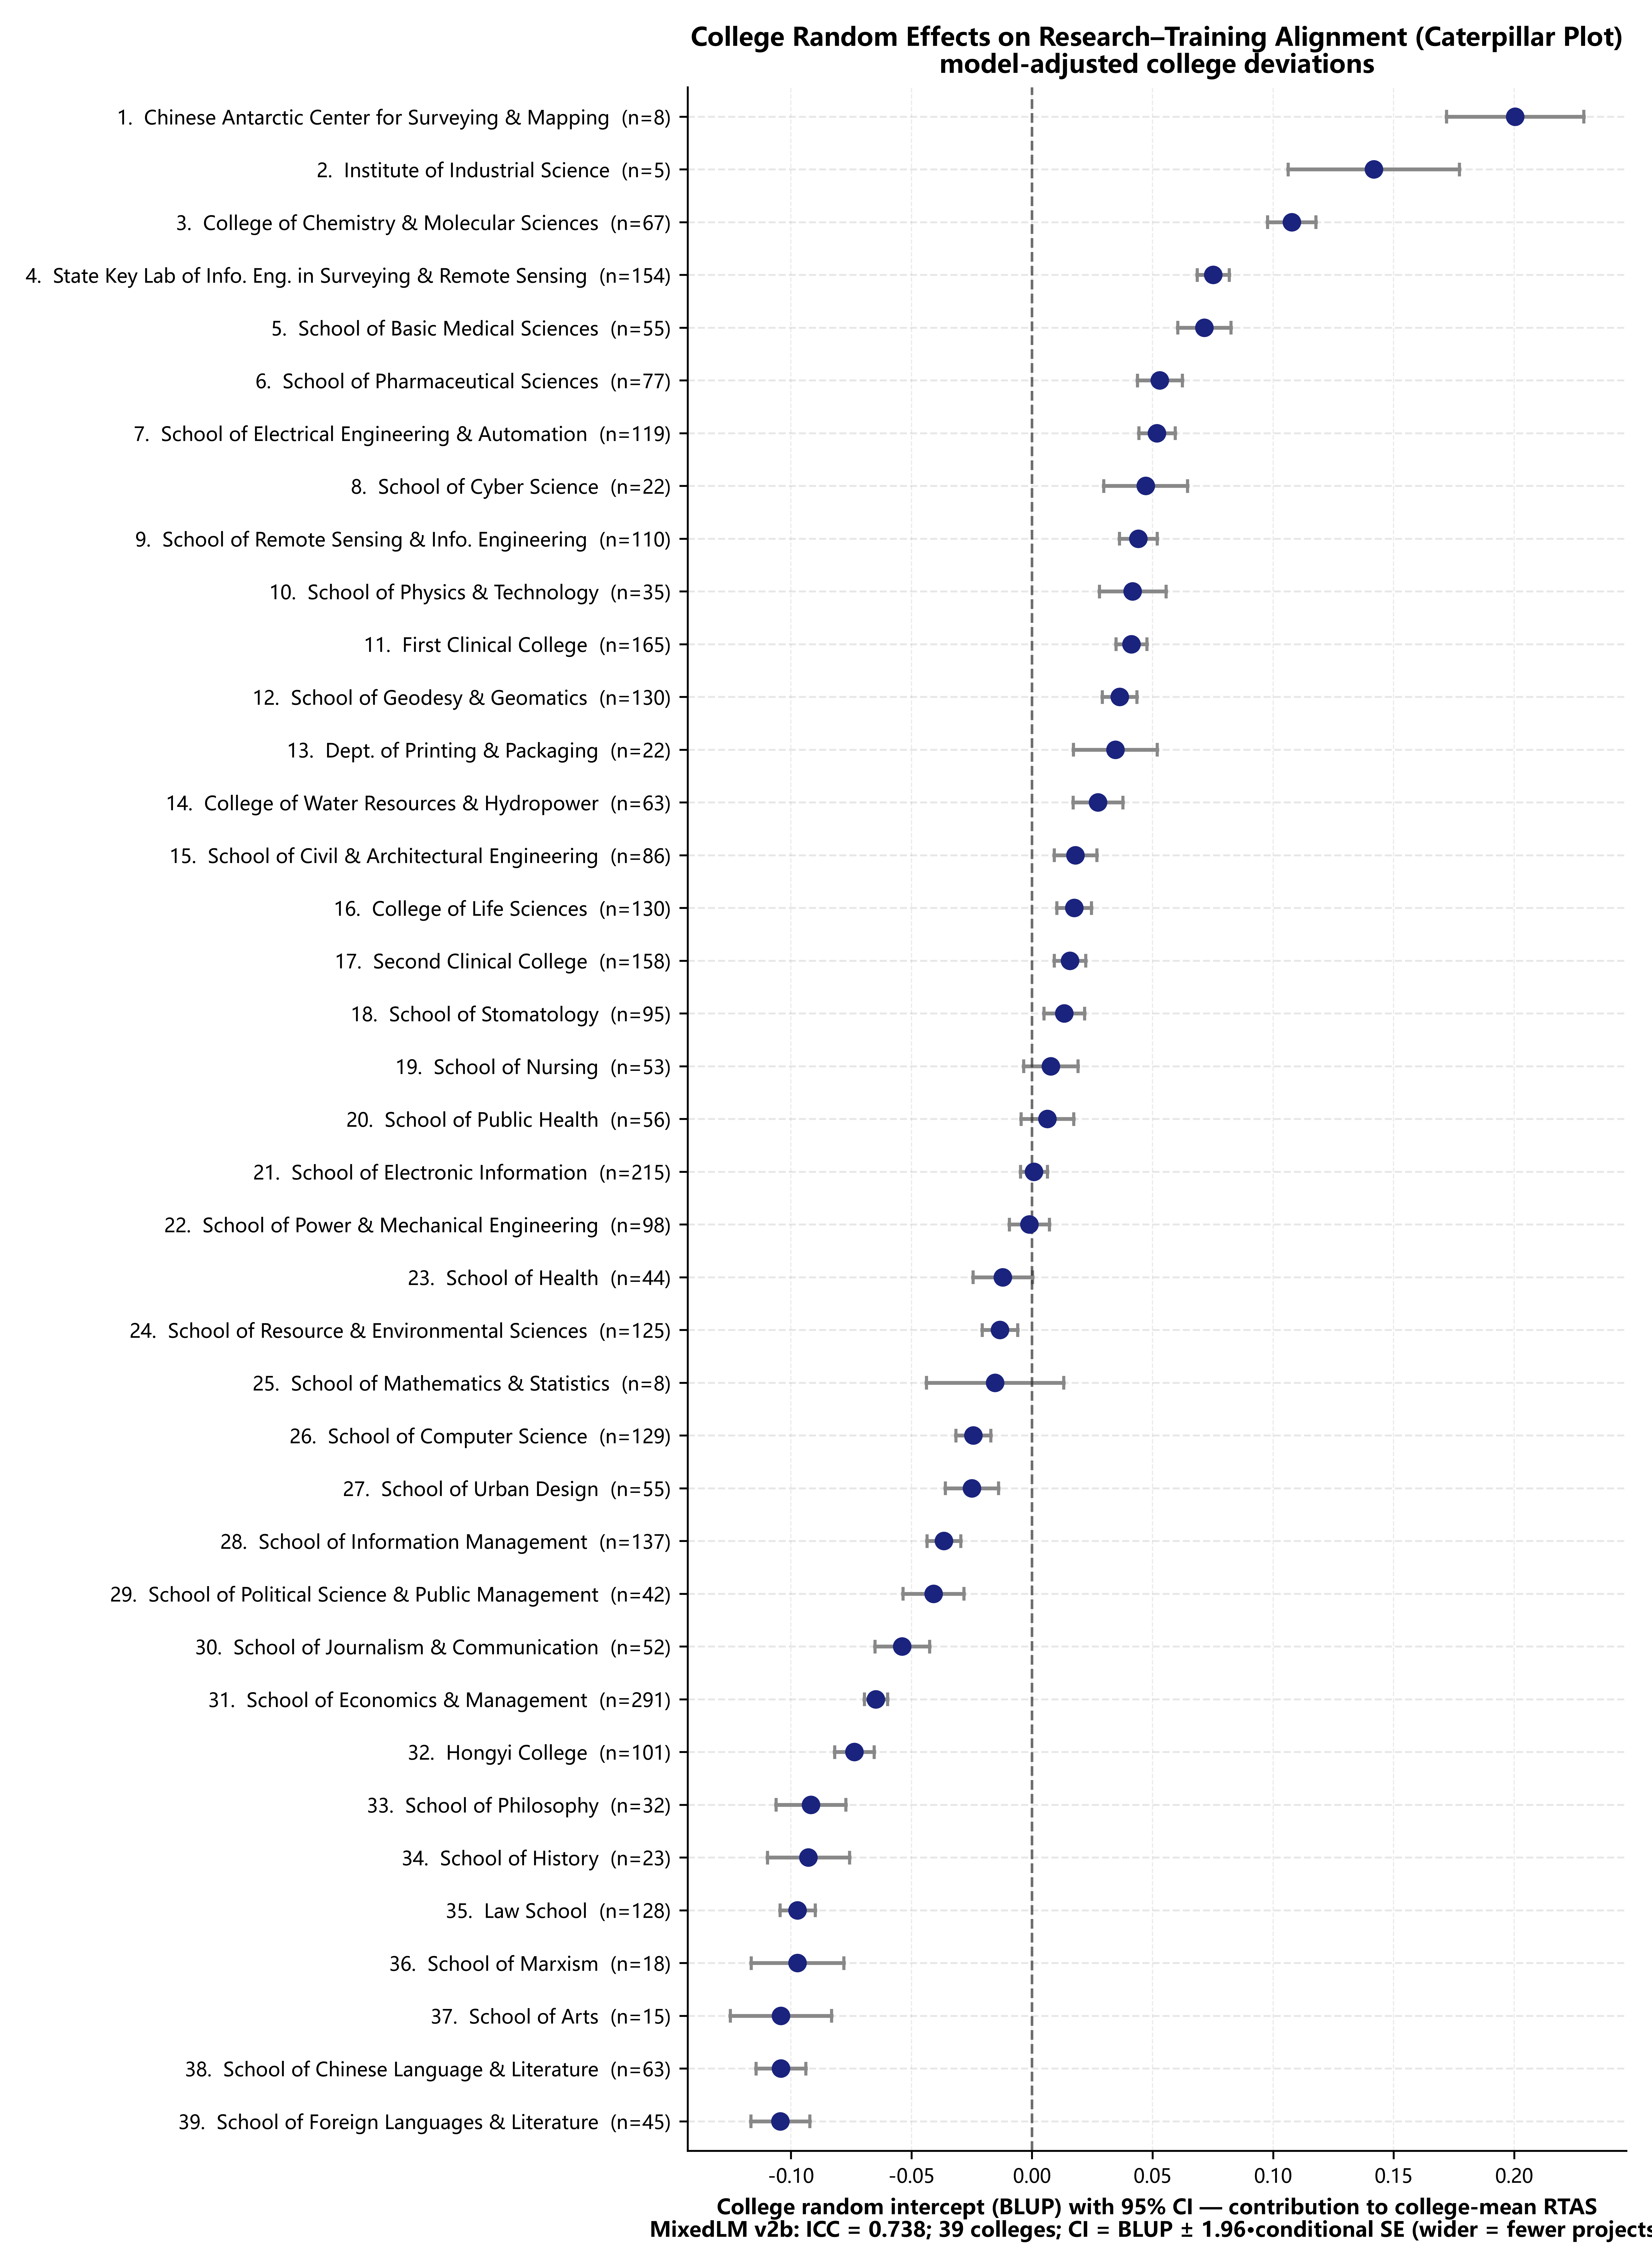
\includegraphics[height=0.84\textheight,keepaspectratio]{Figure5_CollegeCaterpillar.png}
\caption{Model-adjusted college random effects from the primary mixed model. Points are college-level best linear unbiased predictions (BLUPs) and horizontal bars are approximate 95\% conditional intervals. The full project dataset contains 40 colleges; the primary complete-case MixedLM contains 39. These BLUP intervals are descriptive and are not simultaneous or multiple-comparison-adjusted tests. College effects reflect organizational and disciplinary context and are not interpreted as performance rankings.}
\label{fig:college}
\end{figure}

\begin{figure}[H]
\centering

\includegraphics[width=0.96\linewidth]{Figure6_HLM_Forest.png}
\caption{Fixed-effect estimates from the primary mixed model. Points show coefficients and horizontal bars show 95\% confidence intervals. Year is continuous and centered at 2022. Provincial- and national-level confidence intervals cross zero; pre-project publication activity is positively associated with alignment, while prior supervisory load is negatively associated. In the figure, *** denotes $p<.001$ and ns denotes not significant.}
\label{fig:hlm}
\end{figure}

\subsection{Concentration and path dependence (RQ4)}

National project allocation is highly unequal across the 1,834 individual advisors: national-project Gini $=0.746$ and total-project Gini $=0.368$. The top 5\% (92 advisors) hold 31.0\% of national projects, and the top 20\% (366 advisors) hold 71.9\%. Observed supervisory activity is also uneven: 818 advisors (44.6\%) supervise one project, whereas 345 (18.8\%) supervise four or more (mean load 2.314, median 2, maximum 10). Allocation shows year-to-year persistence: in the primary continuous-activity risk set, a national project at $t-1$ is associated with higher odds of another at $t$ (OR $=2.06$, 95\% CI [1.53, 2.76], $p=1.5\times10^{-6}$; 979 advisor-years / 627 advisors). The expanded prior-active risk set gives OR $=2.45$ [1.91, 3.16], $p=3.2\times10^{-12}$ (2,469 advisor-years / 1,560 advisors). At the project level, 560 projects have at least one top-5\% advisor; the mean RTAS difference relative to the remaining projects is small and not statistically distinguishable from zero ($d=0.083$, Welch $p=0.065$). Figure~\ref{fig:matthew} combines the concentration and lagged-persistence results.

\begin{figure}[H]
\centering
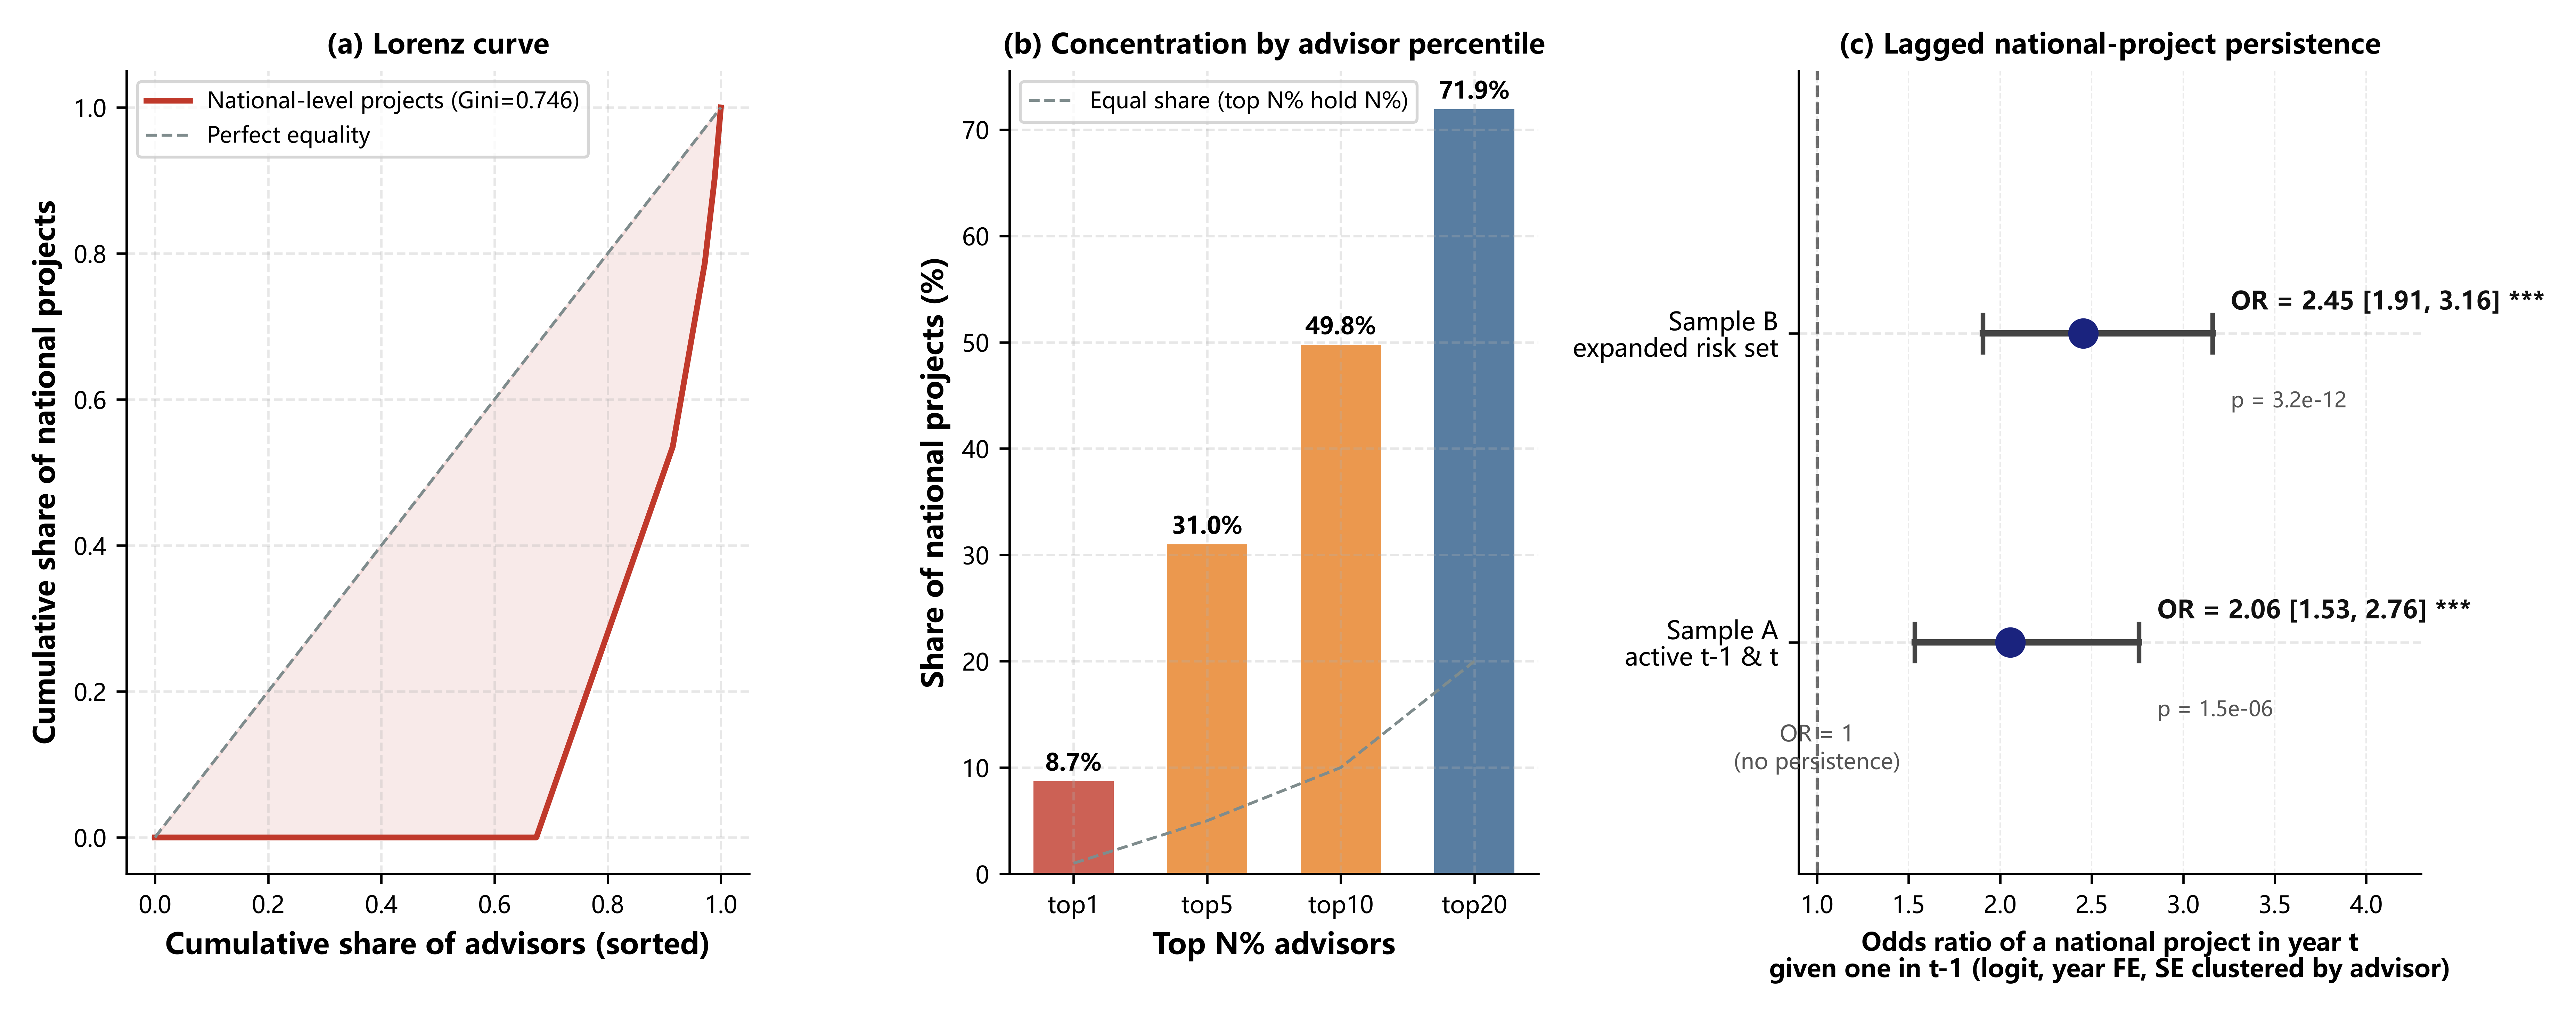
\includegraphics[width=0.99\linewidth]{Figure7_MatthewEffect.png}
\caption{Concentration and lagged persistence in national-level project allocation using individual-advisor units. Panel (a) shows the Lorenz curve for national-project counts (Gini $=0.746$), panel (b) shows the shares of national projects held by the top 1\%, 5\%, 10\%, and 20\% of advisors, and panel (c) shows lagged-logit odds ratios for the primary and expanded risk sets. The vertical reference line in panel (c) is OR $=1$.}
\label{fig:matthew}
\end{figure}

\section{Discussion}

Three patterns organize the findings. First, college context accounts for a large share of RTAS variation, while adjusted funding-level coefficients are close to zero. Among observed project-level covariates, greater pre-project publication activity in the institution-linked OpenAlex corpus is positively associated with RTAS and greater prior supervisory load is negatively associated. The leave-advisor-out sensitivity attenuates the advisor-publication coefficient by approximately 10.5\%, indicating some contribution from mechanical self-overlap while leaving the positive association intact. The single-advisor sensitivity further shows that the substantive fixed-effect conclusions are robust to advisor-clustered inference. National-level allocation is highly concentrated and shows lagged persistence, yet projects linked to top-5\% advisors show only a small mean RTAS difference that is not statistically distinguishable from zero. A capacity-dilution interpretation of the negative load association is therefore plausible but remains non-causal; this reading is compatible with broader mentoring research in which advisor inputs are associated with trainee outcomes \citep{paglis2006adviser}. The concentration and persistence results are also consistent with the cumulative-advantage tradition in the sociology of science \citep{merton1968matthew,merton1988matthewii,allison1982cumulative,diprete2006cumulative}.

Second, static prevalence asymmetry is distinct from temporal lag. Of the 886 clustered topics, 173 are high on the research side but low on the project side, whereas only 10 show the reverse pattern; however, annual onset is definable on both sides for only 29 topics. Treating every HRLT topic as temporally delayed would therefore overread the design.

Third, measurement claims are deliberately bounded. The validity program (independent raters, test--retest, an LLM second rater, lexical baselines, and the post-freeze BGE-M3 benchmark) supports the embedding layer without implying completed construct validity, while quadrant and lag thresholds are reported with sensitivity analyses rather than treated as natural kinds. This restrained interpretation is consistent with responsible-metrics principles and with broader cautions against conflating bibliometric indicators with multidimensional notions of research quality \citep{hicks2015leiden,aksnes2019citations}. RTAS and the scholar-level RT-score answer different questions: the RT-score combines research and teaching performance at the faculty level, whereas RTAS measures project-to-portfolio semantic alignment; they are complementary rather than substitutes.

For research policy, the results suggest that administrative funding tier is less strongly associated with alignment than college context and advisor research activity in this institutional setting. For scientometrics, RTAS illustrates how multilingual sentence embeddings can turn administrative title records into an organizational alignment metric; the same pipeline could be adapted to settings where student project titles and institutional publication portfolios coexist. Recent BERTopic applications further underscore the importance of semantic topic representation and model choice in applied topic mapping \citep{yangkim2025bertopic,benz2025mapping,wang2024bertopic}.

\section{Limitations}
\label{sec:limitations}

\begin{enumerate}
\item \textbf{Observational design.} All associations, including the capacity-dilution interpretation, are non-causal. Stronger directional inference would require non-overlapping longitudinal waves and a design that separates within-unit from between-unit variation.

\item \textbf{Shared bibliographic construction.} For projects after 2020, some papers counted in an advisor's pre-project publication history within the institution-linked corpus can also contribute to the advisor-linked college reference portfolio used to compute RTAS. A leave-advisor-out sensitivity that removed focal-advisor articles attenuated the publication coefficient by approximately 10.5\% while leaving it positive and statistically significant, reducing but not eliminating concern about shared construction. The advisor-output coefficient remains an observational association, not an independent causal effect.

\item \textbf{Titles-only sparsity.} Titles are the only symmetric cross-lingual unit, but they compress semantics; alignment is measured on title distributions, not full texts.

\item \textbf{Linkage coverage.} 58.5\% of articles are advisor-matched to colleges; unmatched articles, including cases with missing affiliations or pinyin ambiguity, are excluded from college reference portfolios. Rule-based name linkage can generate both false-positive and false-negative assignments, so the direction of any resulting bias is uncertain. Author-level identity resolution (e.g., OpenAlex author IDs) remains future work.

\item \textbf{Single institution.} Holding one institutional setting fixed aids within-institution comparison but limits external validity; replication at universities with different disciplinary layouts is required before generalization.

\item \textbf{Prior-supervision history.} The project registry begins in 2020, so prior supervisory load is left-censored at that year; the covariate captures previously observed projects, not an advisor's full pre-2020 supervision history.

\item \textbf{Registry coverage and program tracks.} Official project-type labels exist only for 2021--2024; the 2020 cohort's track (innovation vs entrepreneurship) cannot be classified from the available administrative archive, and the archived 2022 official list contains no university-level entries. The analytic sample consequently pools both tracks (158 identifiable entrepreneurship projects, 4.3\%, which have lower RTAS on average: 0.100 vs 0.135, Cohen $d=-0.49$). Excluding these projects from the mixed model preserves every coefficient sign and significance classification (Table~S1), but a fully track-stratified treatment of the 2020 cohort is not possible from the available records.

\item \textbf{Within-year ordering.} RTAS reference portfolios include articles from the focal calendar year $t$. Because the analysis is annual, it does not establish whether a same-year article preceded or followed the project's approval date; RTAS should therefore be interpreted as contemporaneous annual alignment rather than strict within-year temporal precedence.

\item \textbf{Advisor-level dependence and multiple membership.} The primary mixed model accounts for clustering by college but does not include a separate advisor random effect. A single-advisor sensitivity using college fixed effects and advisor-clustered standard errors preserved all substantive fixed-effect conclusions, including under the college $\times$ advisor homonym guard. However, 528 co-supervised projects have no primary-advisor designation, so a full multiple-membership model is not estimated.

\item \textbf{Low lag definition rate.} Only 3.27\% of topics have definable lags; LRHT/LRLT lags are undefined in this corpus, so no ``outdated training content'' claim is possible here. A curriculum-syllabus text audit could help address this gap.

\item \textbf{Measure sensitivity.} College-level RTAS mixes organizational context with sensitivity to disciplinary specialization, portfolio breadth, title-language conventions, and heterogeneity; college-level differences should not be interpreted as performance rankings.

\item \textbf{Encoder scope.} BGE-M3 was benchmarked post-freeze on the same 150-pair reference set and did not improve pairwise validity relative to MiniLM. Because the comparison was limited to the validation set rather than a full-pipeline re-estimation, MiniLM remains the frozen primary encoder and the BGE-M3 result should be interpreted as a targeted robustness check rather than an exhaustive encoder comparison.

\item \textbf{Granularity.} $K=886$ is corpus-determined (HDBSCAN), not a theoretically fixed granularity; the topic count should not be interpreted substantively in isolation.
\end{enumerate}

\section{Conclusion}

We introduced RTAS, a project-level, cross-lingual semantic alignment measure, and applied it to 3,714 undergraduate innovation projects and 56,901 articles at Wuhan University. Alignment rises with project funding level in raw comparisons, but adjusted funding-level coefficients are not statistically distinguishable from zero once college context and advisor characteristics are modeled. Research-side and project-side topic prevalence are markedly asymmetric (173 high-research/low-project vs 10 low-research/high-project topics), and temporal lags are definable for only 29 topics. Of these, 24 fall in the high-research/low-project stratum, within which the median lag is $+0.5$ years. National project allocation is highly concentrated and shows lagged persistence, yet projects linked to top-5\% advisors show only a small mean alignment difference that is not statistically distinguishable from zero; advisors' pre-project publication activity in the institution-linked OpenAlex corpus is positively associated with alignment and prior supervisory load is negatively associated, a pattern compatible with capacity dilution but not causally identified. The analytic workflow emphasizes reproducibility and bounded interpretation; RTAS indexes alignment, not quality.

\section*{Statements and Declarations}

\textbf{Funding.} [To be completed.]

\textbf{Conflicts of interest.} The authors declare no competing interests.

\textbf{Ethics approval.} The study analyzes institutional administrative records and publicly retrievable bibliographic metadata. [The applicable institutional ethics/IRB determination is to be completed before submission.]

\textbf{Data availability.} (i) \emph{Publicly retrievable layer:} OpenAlex article records are publicly retrievable through the documented institutional query (Wuhan University; institution I37461747; type=article; cursor pagination). The primary 2020--2024 corpus was retrieved on September 3, 2026; the auxiliary 2017--2019 corpus used only for prior advisor covariates was retrieved on September 4, 2026. (ii) \emph{Restricted layer:} the undergraduate project records were compiled from administrative records supplied by teaching administrators in the 40 colleges and consolidated into a unified study dataset. Because the records contain personal information, including advisor names, the raw data cannot be publicly redistributed. (iii) \emph{Derived outputs:} non-identifying derived outputs and code (frozen aggregation tables, quadrant and lag summaries, model estimates, and figure scripts) are maintained in the project repository:
\url{https://github.com/victoryangcw/RTAS-knowledge-diffusion}, currently private and intended for public release. These materials can reproduce the reported analyses from shareable frozen derived inputs; complete independent reconstruction requires equivalent access to the restricted institutional records.

\textbf{Code availability.} See Data availability (iii); all analyses are scripted end-to-end from frozen analysis inputs.

\textbf{Author contributions.} [To be completed.]

\printbibliography


% =========================================================
% SUPPLEMENTARY MATERIAL
% Online Resource 1
% =========================================================

\clearpage

% Supplementary pages: S1, S2, ...
\renewcommand{\thepage}{S\arabic{page}}
\setcounter{page}{1}

% Supplementary figures: S1, S2, S3a, S3b, S4
\renewcommand{\thefigure}{S\arabic{figure}}
\setcounter{figure}{0}

% Supplementary tables, if added later: S1, S2, ...
\renewcommand{\thetable}{S\arabic{table}}
\setcounter{table}{0}


\begin{center}
{\LARGE\bfseries Supplementary Material (Online Resource 1)}

\vspace{0.8em}

{\large
Measuring Research--Training Semantic Alignment:
Project-Level Cross-Lingual Embeddings, Topic Prevalence
Asymmetries, and Resource Concentration in Undergraduate
Innovation Programs
}

\vspace{0.8em}

Author Name\\
Affiliation to be completed\\
Corresponding author: email@domain.edu
\end{center}

\vspace{1em}

\section*{Supplementary Figures}


% ---------------------------------------------------------
% Figure S1
% ---------------------------------------------------------

\begin{figure}[H]
\centering
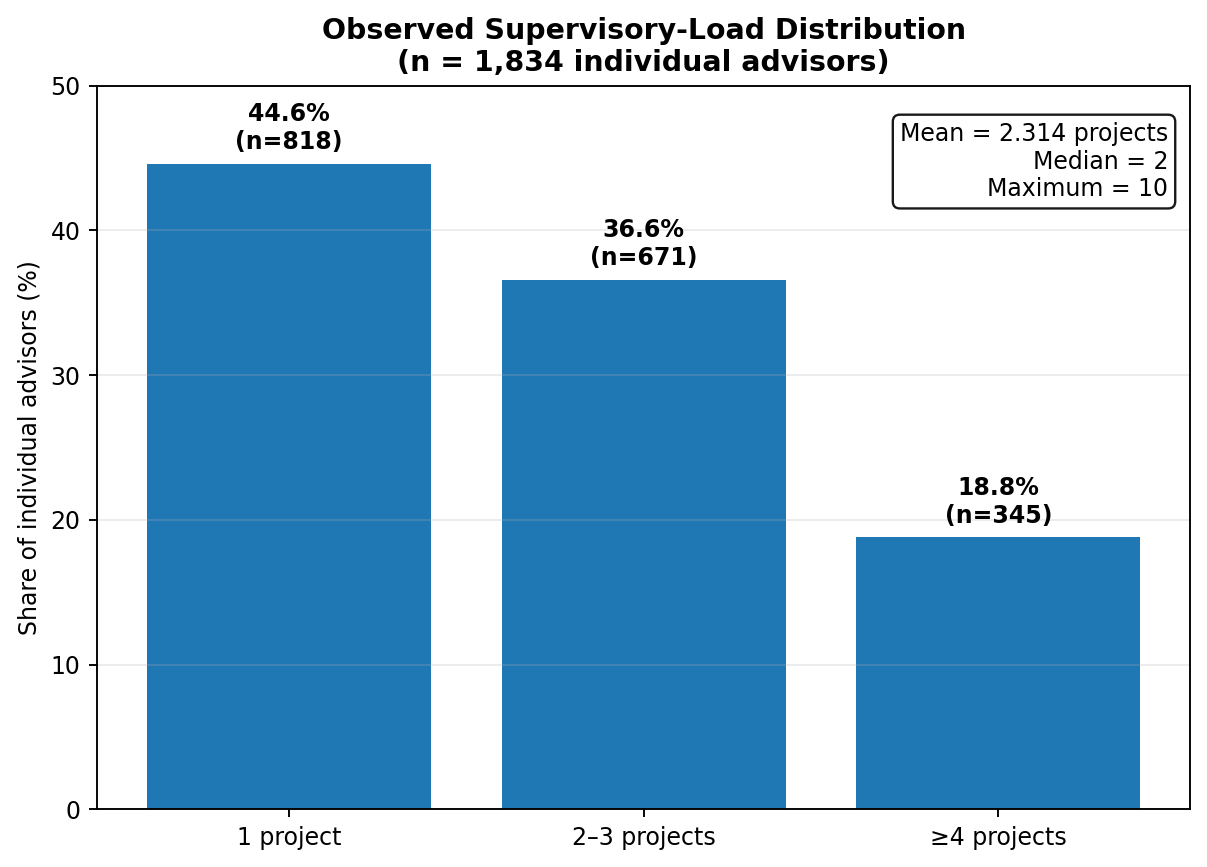
\includegraphics[width=0.82\linewidth]{FigureS1_SupervisorLoad.png}
\caption{Observed supervisory-load distribution among 1,834 individual advisors after multi-advisor project fields were split using the same rules as the main analysis. Counts are based on distinct advisor--project links in the 2020--2024 registry. The 2--3-project category is the complement of the one-project and $\ge4$-project groups; mean load is 2.314 projects, median 2, and maximum 10.}
\label{fig:s1}
\end{figure}


% ---------------------------------------------------------
% Figure S2
% ---------------------------------------------------------

\begin{figure}[H]
\centering
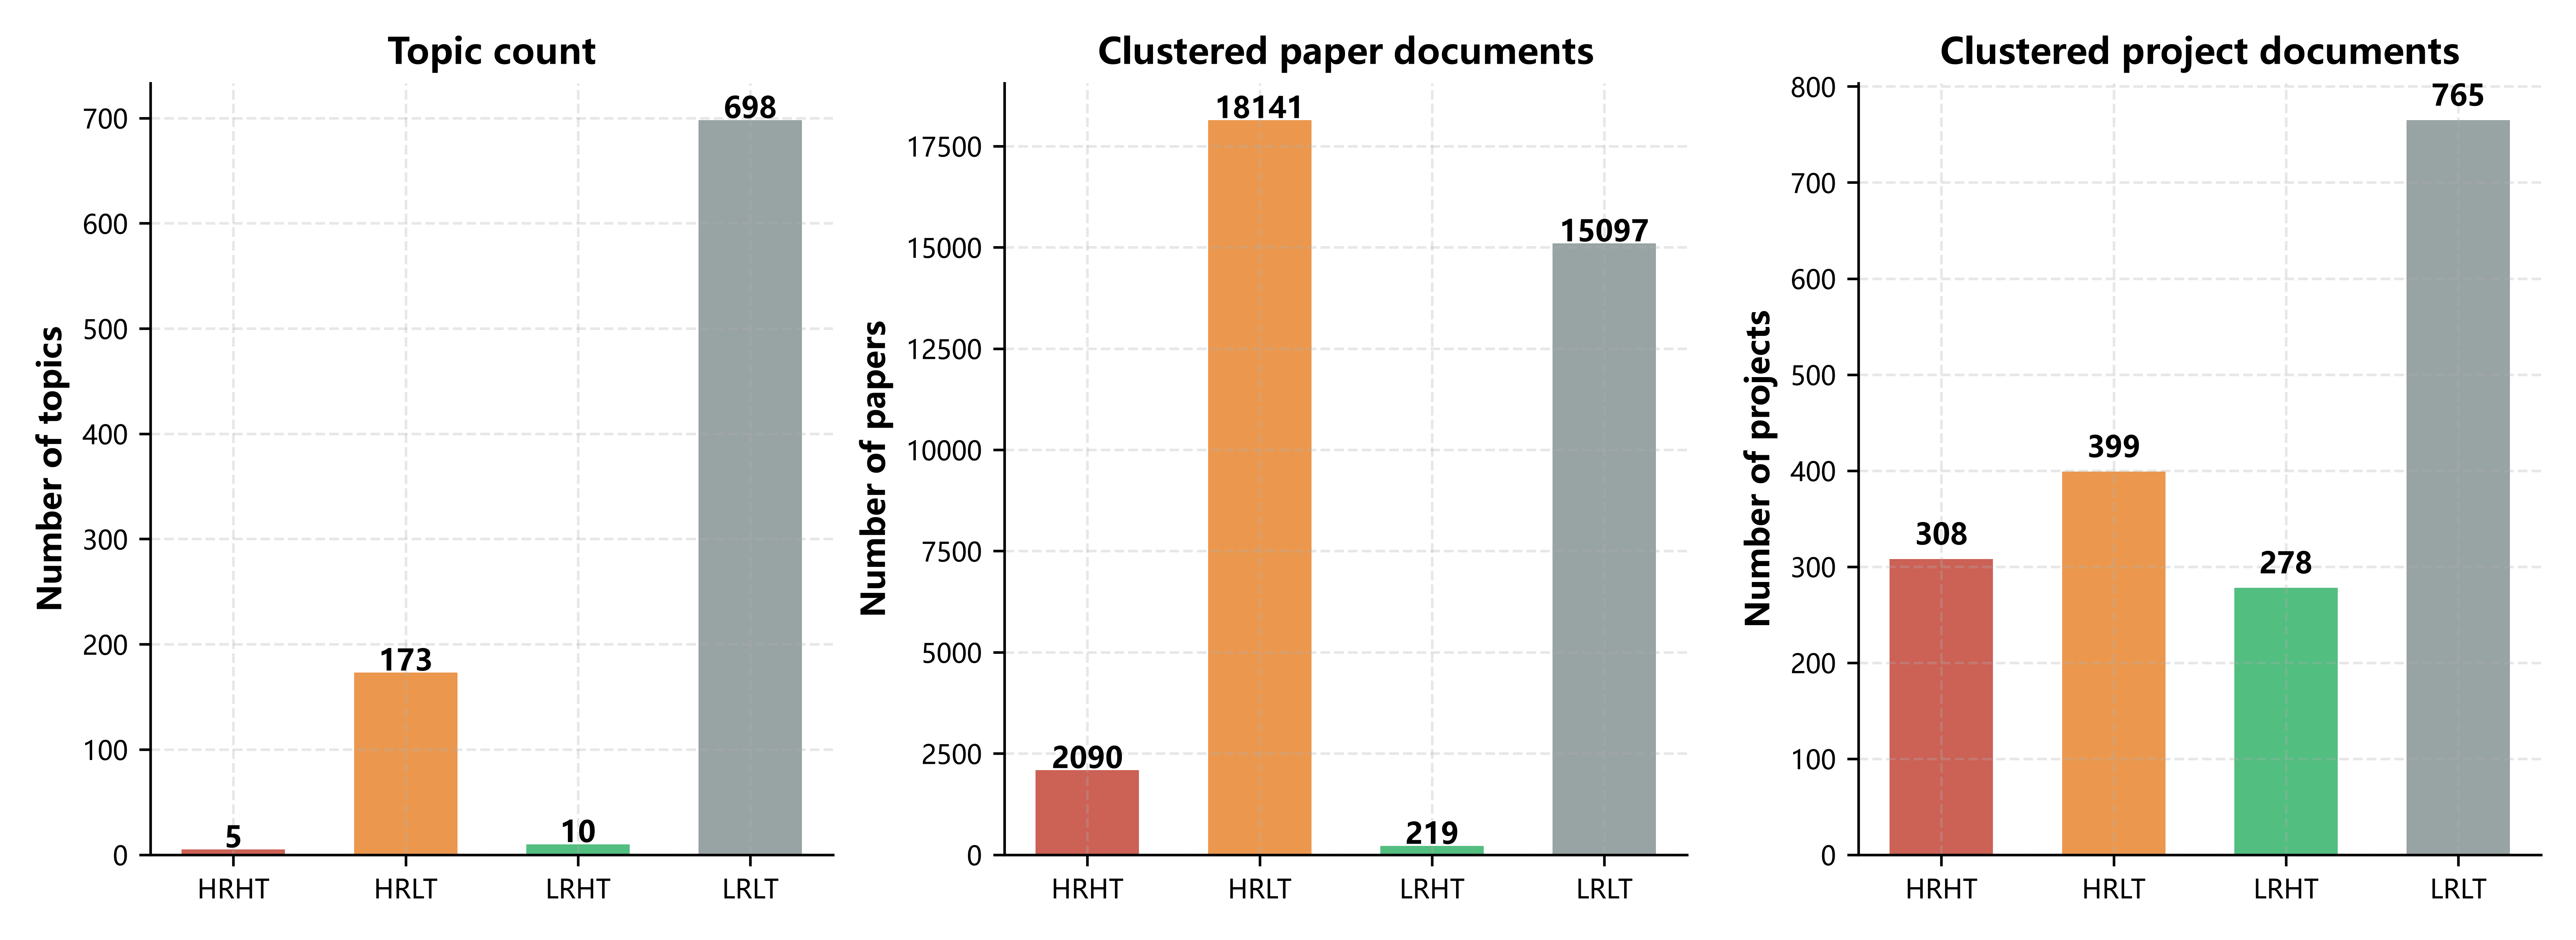
\includegraphics[width=0.98\linewidth]{FigureS2_QuadrantSummary.png}
\caption{Four-quadrant summary for clustered documents. Bars count documents assigned to the 886 non-outlier topics; BERTopic outliers are excluded from the quadrant counts. The prevalence thresholds used to classify topics are defined against the full article and project corpora, as specified in the main text.}
\label{fig:s2}
\end{figure}


% ---------------------------------------------------------
% Figure S3a
% ---------------------------------------------------------

\begin{figure}[H]
\centering
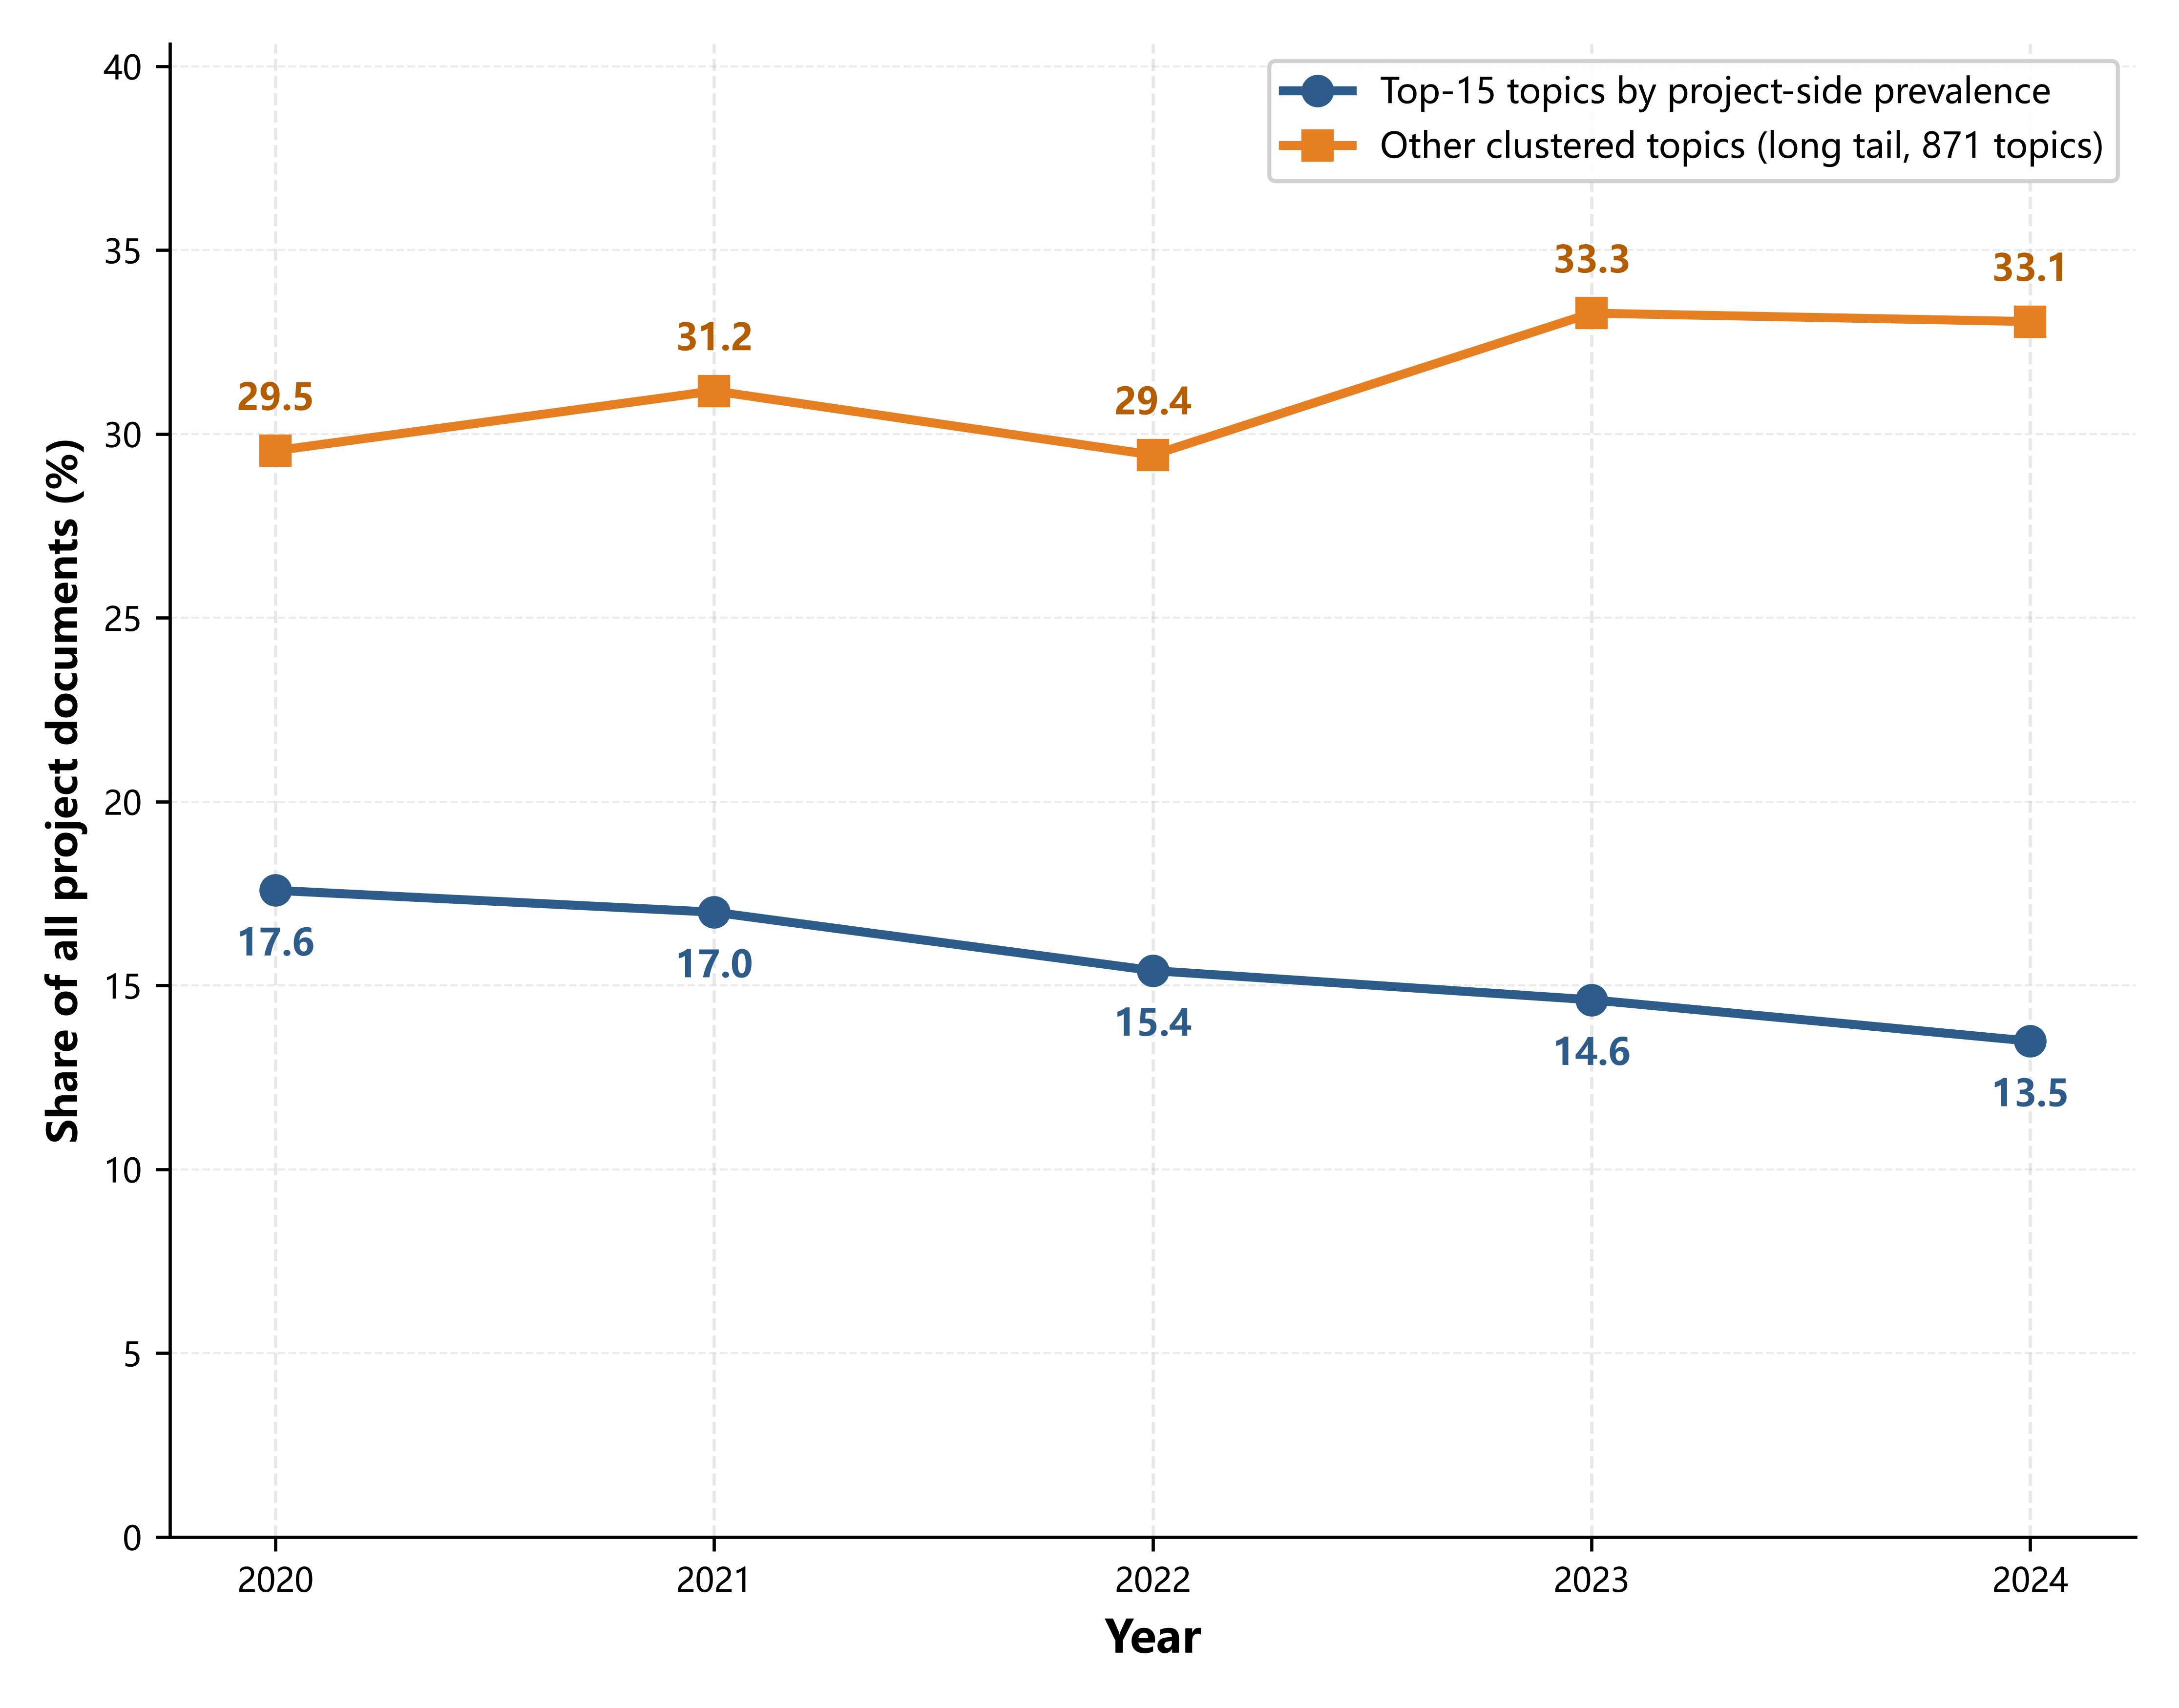
\includegraphics[width=0.92\linewidth]{FigureS3a_TopicTrend.png}
\caption*{\textbf{Figure S3a.} Topic dynamics in undergraduate innovation projects, 2020--2024: aggregate share of the 15 most prevalent clustered topics versus all other clustered topics. Annual denominators include all projects, whereas BERTopic outliers are absent from both plotted numerators; consequently, the two lines do not sum to 100\%. This is a prevalence-share comparison, not a formal diversity index.}
\end{figure}


% ---------------------------------------------------------
% Figure S3b
% ---------------------------------------------------------

\begin{figure}[H]
\centering
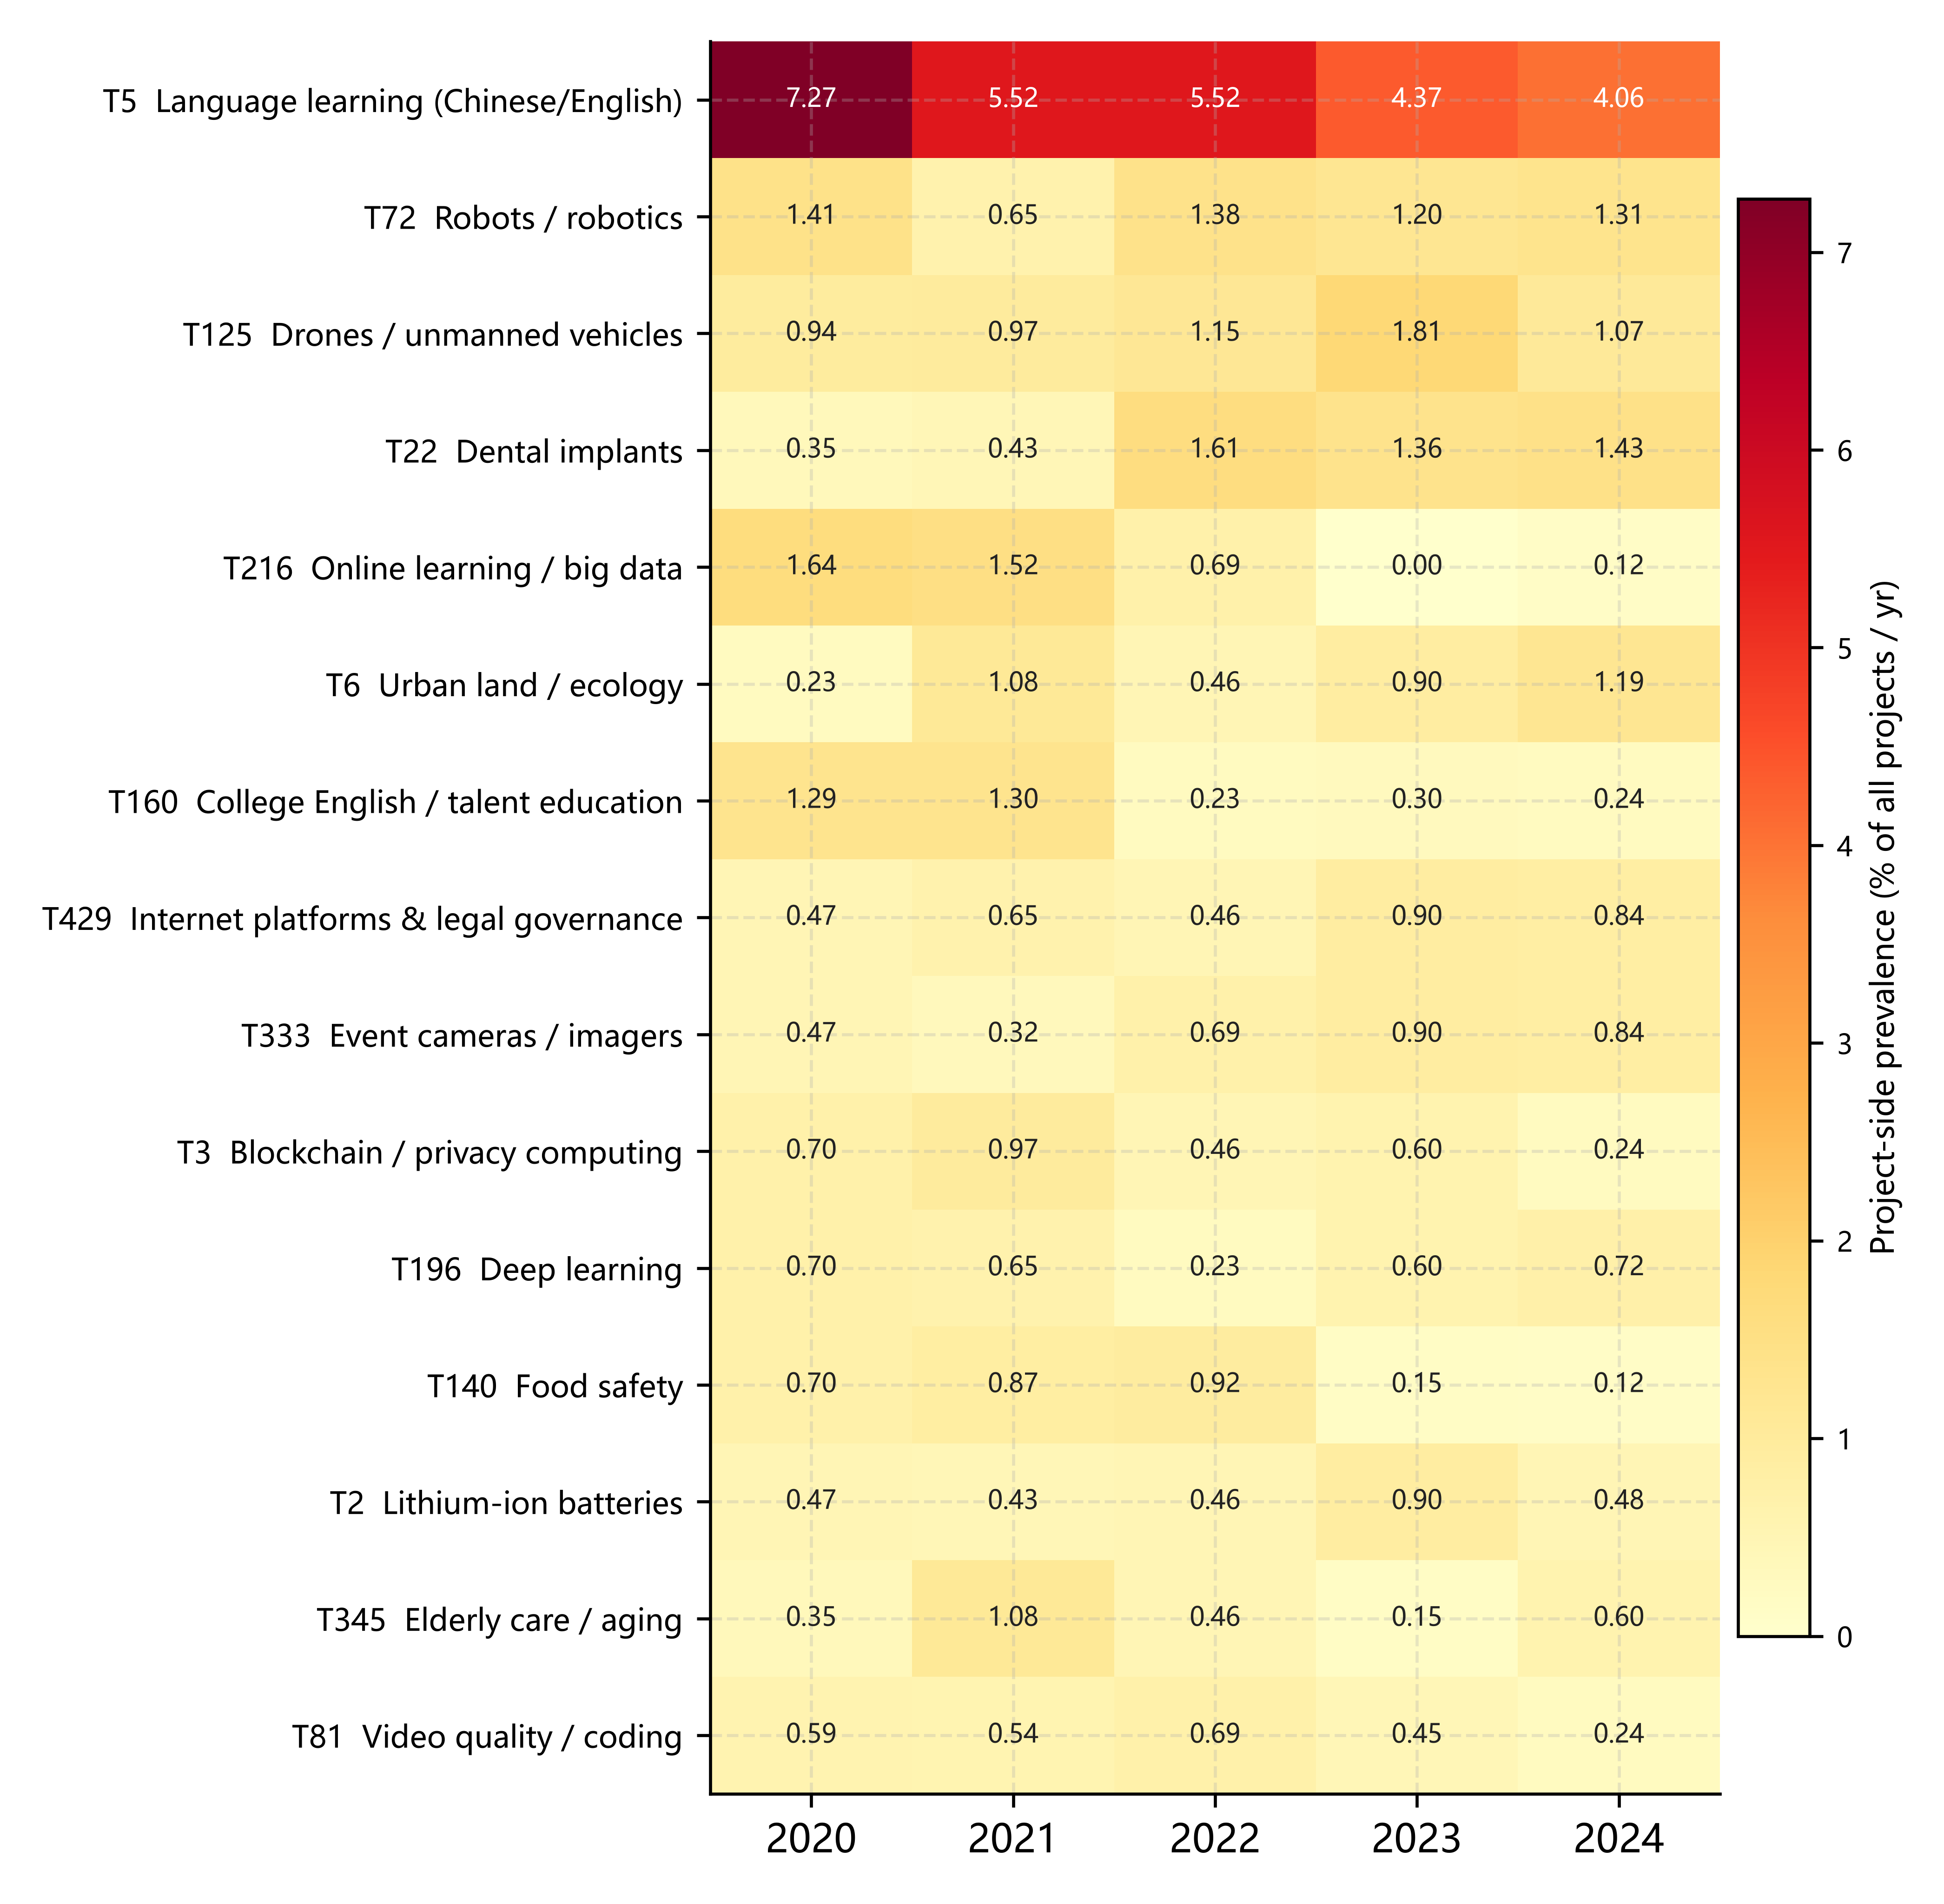
\includegraphics[width=0.92\linewidth]{FigureS3b_TopicHeatmap.png}
\caption*{\textbf{Figure S3b.} Top-15 project-side topic prevalence by year, 2020--2024.}
\end{figure}


% ---------------------------------------------------------
% Figure S4
% ---------------------------------------------------------

\setcounter{figure}{3}
\begin{figure}[H]
\centering
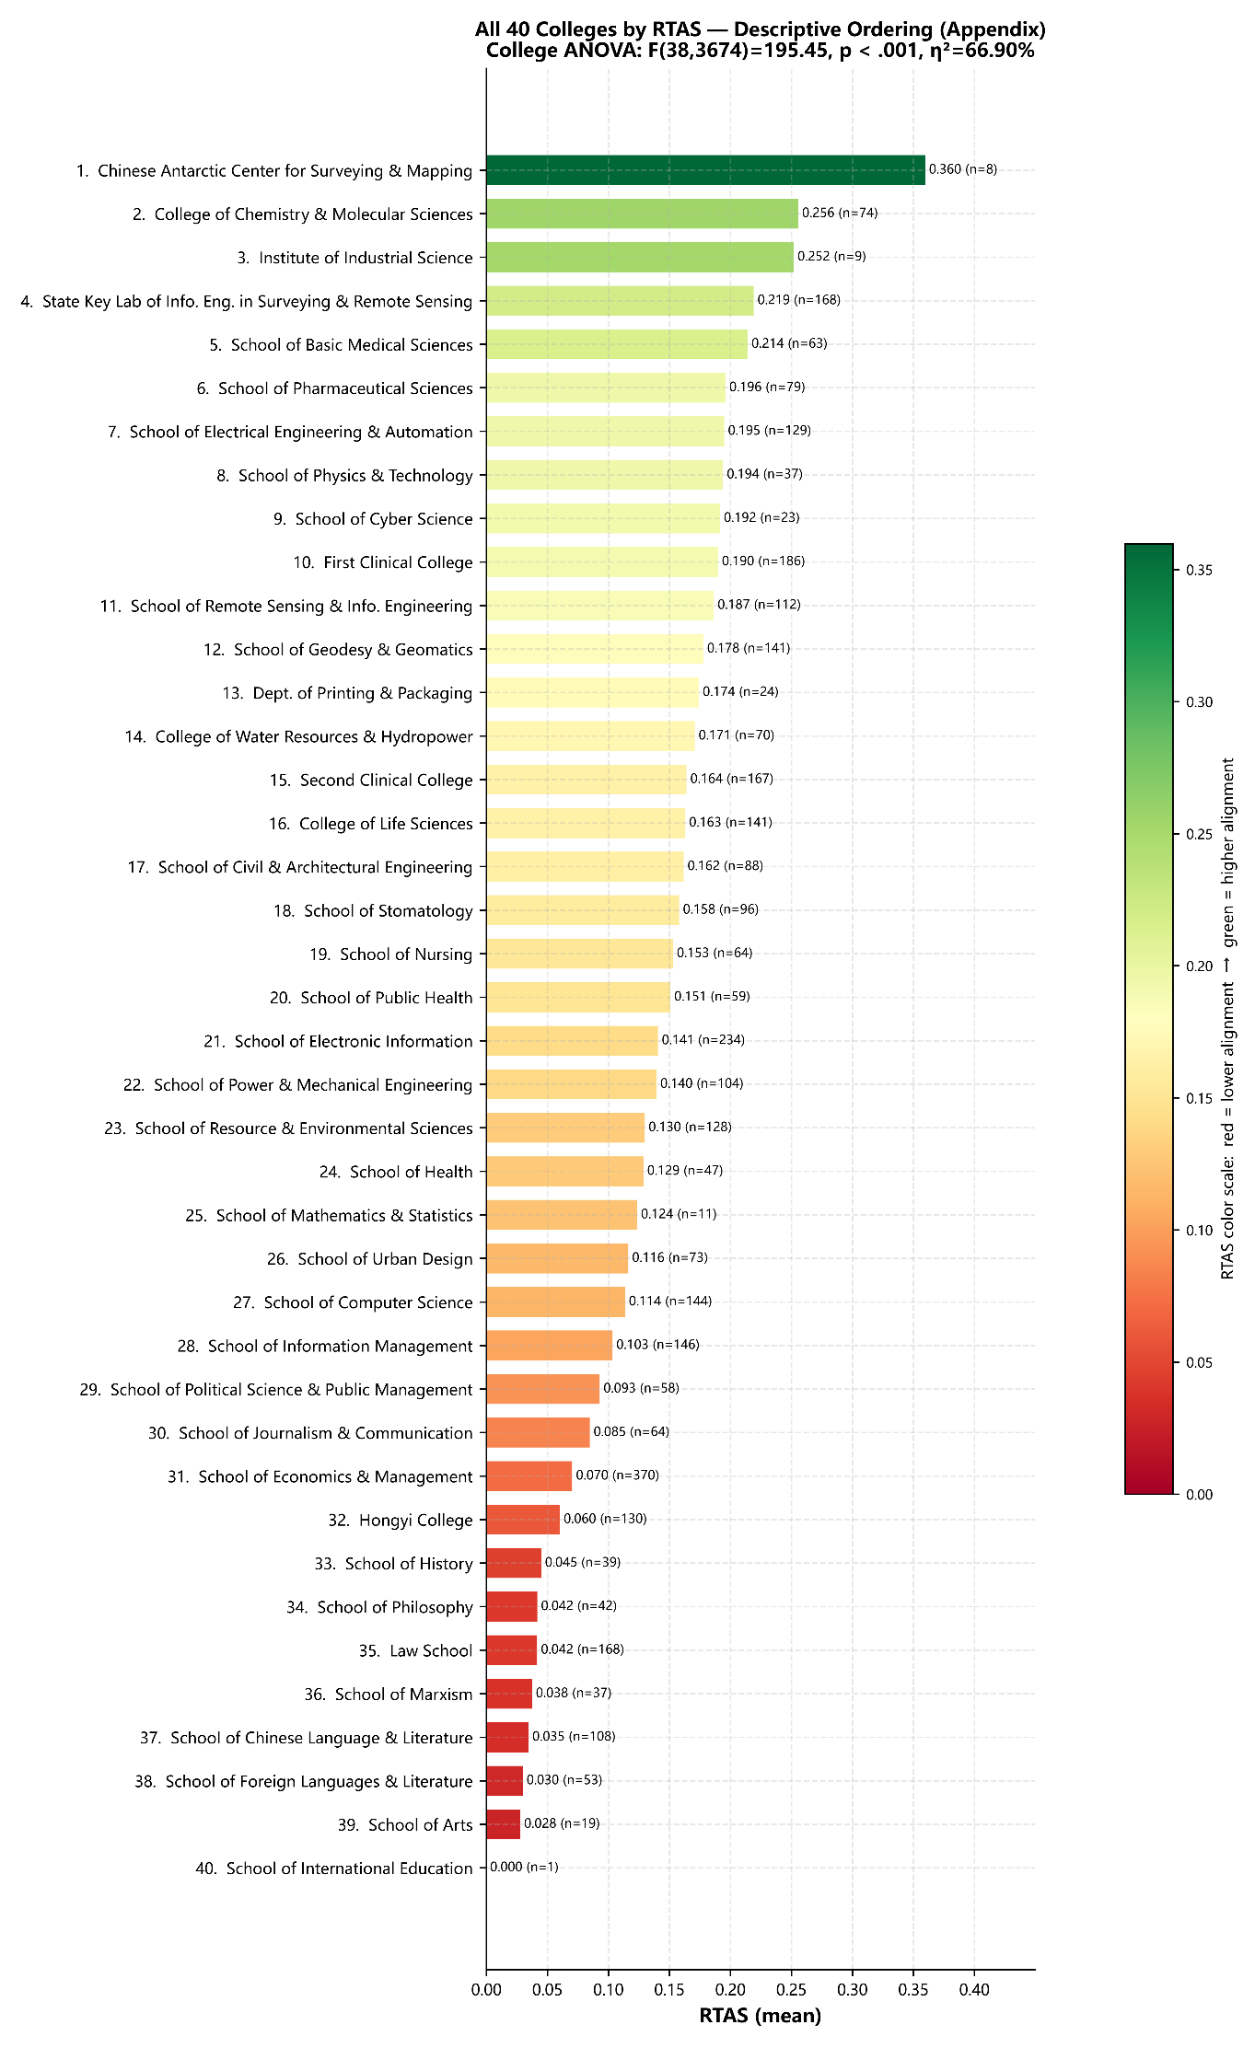
\includegraphics[height=0.88\textheight,keepaspectratio]{FigureS4_CollegeRTAS_Full40.png}
\caption{Descriptive RTAS means for all 40 colleges using the full project dataset. The one-way college ANOVA shown in the figure uses 39 colleges because the single-project college cannot contribute a within-group variance estimate; this ANOVA effect size is distinct from the adjusted mixed-model ICC in the main text. The ordering is descriptive and should not be interpreted as a performance ranking.}
\label{fig:s4}
\end{figure}


\section*{Supplementary Tables}

% ---------------------------------------------------------
% Table S1
% ---------------------------------------------------------

The official 2021--2024 approval lists classify projects as innovation training or entrepreneurship training/practice. Matching on (year, normalized title) identifies 158 unique entrepreneurship projects inside the frozen 3,714-row dataset (4.3\%; 74/23/26/35 across 2021--2024; 53 university-, 64 provincial-, and 41 national-level). These projects have lower alignment than the remaining 3,556 projects: mean RTAS $=0.100$ (SD $=0.053$) versus $0.135$ (SD $=0.073$); Welch $t=-7.90$, $p<0.001$, Cohen $d=-0.49$ (pooled SD). Table~S1 re-estimates the frozen random-intercept specification (REML, clustered by college, covariates taken from the frozen dataset unchanged) after excluding these 158 projects: the complete-case sample falls from 3,231 to 3,085 projects, ICC changes from 0.7376 to 0.7373, every coefficient retains its sign and significance classification, and the funding-level indicators remain non-significant. The 2020 cohort is retained in both fits because no type-labeled official registry exists for that year.

\begin{table}[H]
\centering
\caption{Sensitivity of the Table~6 mixed model to excluding the 158 officially typed entrepreneurship projects (2021--2024).}
\label{tab:s1}
\begin{tabular}{lrrrr}
\toprule
& \multicolumn{2}{c}{Primary ($N=3{,}231$)} & \multicolumn{2}{c}{Excluding entrepreneurship ($N=3{,}085$)}\\
\cmidrule(lr){2-3}\cmidrule(lr){4-5}
Predictor & $\beta$ & $p$ & $\beta$ & $p$\\
\midrule
Provincial vs university & 0.00062 & 0.720 & 0.00085 & 0.627\\
National vs university & $-0.00162$ & 0.452 & $-0.00205$ & 0.357\\
Year (per year; centered 2022) & 0.00313 & $<0.001$ & 0.00293 & $<0.001$\\
Advisor prior 3y works, $\log(1+x)$ & 0.00427 & $<0.001$ & 0.00480 & $<0.001$\\
Advisor prior supervised projects, $\log(1+x)$ & $-0.00629$ & $<0.001$ & $-0.00567$ & $<0.001$\\
\midrule
ICC & 0.7376 & & 0.7373 & \\
Number of colleges & 39 & & 39 & \\
\bottomrule
\end{tabular}

\vspace{1mm}
\footnotesize Same specification as Table~6: RTAS $\sim$ provincial $+$ national $+$ year $+$ $\log(1+\text{prior 3y works})$ $+$ $\log(1+\text{prior supervised projects})$, random intercept by college, REML. Entrepreneurship projects are identified from the official 2021--2024 project-type field; 2020 track membership is unobservable, so no 2020 project is excluded.
\end{table}


\end{document}